%!TEX root = ../thesis.tex
%*******************************************************************************
%****************************** Literature Review Chapter **********************
%*******************************************************************************
\chapter{Background Theory} \label{chapter:Literature Review}

\graphicspath{{Chapter_LR/Figs/}}
This chapter lays down the fundamental theories of optoelectronics and search algorithms, which are essential to the research outlined in the later chapters of this thesis.


\section{The Nature of Light}
\subsection{Wave-Particle Duality}
The problem of how light propagates has been troubling scientists for centuries. In the 17th century, Sir Isaac Newton made a significant step. He proposed that light consists of particles, or `corpuscles', with a mass varying with colour, which explained phenomena such as reflection and refraction \cite{Newton1704}. In contrast, Christiaan Huygens, a contemporary of Newton, demonstrated that light behaves as a wave, as it is capable of diffraction, which is the bending of light around the edge of an object, leading to the non-sharp edges of shadows \cite{Huygens1690}.

\begin{figure}[H]
	\centering
	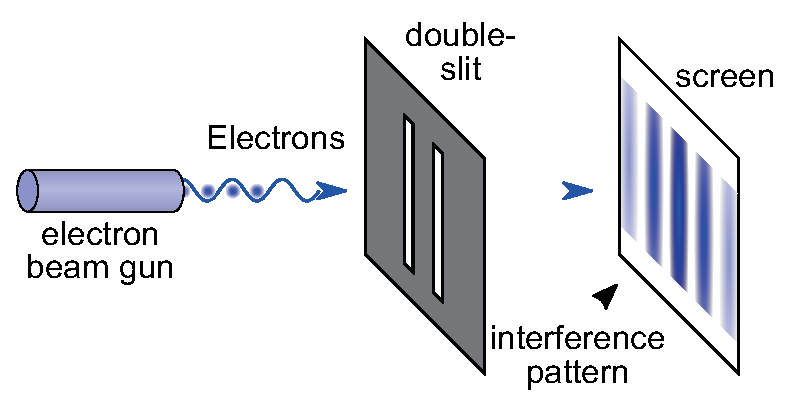
\includegraphics[width=0.7\textwidth]{Double-slit.eps}
	\caption{An illustration of the Young's Double-slit experiment \cite{Kalliauer2017}}
	\label{fig:Double-slit.eps}
\end{figure}

The wave theory gained significant support in the early 19th century through the experiments by Thomas Young. Young's double-slit experiment in 1801 provided clear evidence of the wave nature of light by showing that light passing through two slits creates an interference pattern on a screen \cite{Young1802}, as illustrated in \cref{fig:Double-slit.eps}. Augustin-Jean Fresnel further advanced the wave theory by developing a comprehensive mathematical framework to describe light as a wave, explaining phenomena such as polarization and the diffraction of light \cite{Fresnel1826}.

This understanding was further reinforced by James Clerk Maxwell in the mid-19th century. In 1864, James Clerk Maxwell organised a set of four equations describing the space and time dependence of the electromagnetic field, which are:
\begin{align}
  \nabla \times \mathbb{E} & = -\frac{\partial \mathbb{B}}{\partial t}             \label{eq:maxwell1} \\
  \nabla \times \mathbb{H} & = \mathbb{J} + \frac{\partial \mathbb{D}}{\partial t} \label{eq:maxwell2} \\
  \nabla \cdot \mathbb{D}  & = \rho                                                \label{eq:maxwell3} \\
  \nabla \cdot \mathbb{B}  & = 0 \label{eq:maxwell4}
\end{align}
where $\mathbb{D}$ is the electric flux density, $\mathbb{E}$ is the electric field intensity, $\mathbb{B}$ is the magnetic flux density, $\mathbb{H}$ is the magnetic field intensity, $\rho$ is the volume charge density, and $\mathbb{J}$ is the current density \cite{Daintith2009}.

And the relation between $\mathbb{D}$ and $\mathbb{E}$ and between $\mathbb{B}$ and $\mathbb{H}$ for linear materials are:
\begin{align}
  \mathbb{B} & = \mu \mathbb{H}      \\
  \mathbb{D} & = \epsilon \mathbb{E}
\end{align}
where $\mu$ is the magnetic permeability and $\epsilon$ is the dielectric permittivity of the material \cite{Wilkinson2017}.

Maxwell's equations unified electricity and magnetism into a single theory of electromagnetism, predicting that light is an electromagnetic wave that propagates through space \cite{Maxwell1865}.

Despite the success of the wave theory, it could not explain all light-related phenomena. The early 20th century brought a pivotal development with Albert Einstein's explanation of the photoelectric effect. In 1905, Einstein proposed that light also behaves as particles, or `quanta' (later called photons), which could eject electrons from a metal surface when light is shone upon it \cite{Einstein1905}. This particle nature of light was critical in explaining observations that wave theory alone could not address and earned Einstein the Nobel Prize in Physics in 1921.

These discoveries collectively revealed that light exhibits both wave and particle properties, depending on the experimental context. This wave-particle duality became a cornerstone of quantum mechanics, fundamentally altering human's understanding of the nature of light. Although to date, it is still not yet known what light exactly is, it is now known how light behaves.

\subsection{Wave Equation}
To mathematically describe the propagation of light in free space (i.e. in absence of free charge), the Maxwell equations in \cref{eq:maxwell1} - \cref{eq:maxwell4} can be simplified as:
\begin{align}
  \nabla \times \mathbb{E}         & = -\mu \frac{\partial \mathbb{H}}{\partial t}     \label{eq:simplified_maxwell1} \\
  \nabla \times \mathbb{H}         & = \epsilon \frac{\partial \mathbb{E}}{\partial t} \label{eq:simplified_maxwell2} \\
  \nabla \cdot \epsilon \mathbb{E} & = 0                                               \label{eq:simplified_maxwell3} \\
  \nabla \cdot \mu \mathbb{H}      & = 0 \label{eq:simplified_maxwell4}
\end{align}

Taking the curl on both the left and right hand sides of \cref{eq:simplified_maxwell1}, and using the vector identity of $\nabla \times (\nabla \times \textbf{u}) = \nabla(\nabla \cdot \textbf{u}) - \nabla^2 \textbf{u}$, we get:
\begin{align}
  \nabla \times (\nabla \times \mathbb{E})               & = -\nabla \times (\mu \frac{\partial \mathbb{H}}{\partial t}) \label{eq:wave_equation_derivation1} \\
  \nabla (\nabla \cdot \mathbb{E}) - \nabla^2 \mathbb{E} & = -\frac{\partial}{\partial t} \nabla \times (\mu \mathbb{H}) \label{eq:wave_equation_derivation2}
\end{align}

Then, by substituting \cref{eq:simplified_maxwell2} and \cref{eq:simplified_maxwell3} in, \cref{eq:wave_equation_derivation2} becomes:
\begin{equation}
  -\nabla^2 \mathbb{E} = -\frac{\partial}{\partial t} (\mu \epsilon \frac{\partial \mathbb{E}}{\partial t}) \label{eq:wave_equation_derivation3}
\end{equation}

Hence, we have a generic form of wave equation, relating the space and time domain relation of electromagnetic waves propagating in free space:
\begin{equation}
  \nabla^2 \mathbb{E} = \mu \epsilon \frac{\partial^2 \mathbb{E}}{\partial t^2} \label{eq:wave_equation}
\end{equation}

A valid solution to \cref{eq:wave_equation} is:
\begin{equation}
  \mathbb{E} = \mathbb{E}_0 e^{j(\omega t - k r)} \label{eq:wave_equation_solution}
\end{equation}
where $\omega$ is the angular velocity of the wave, $t$ is time, $r$ is the propagation distance and $k$ is called the wave number ($k=\frac{2\pi}{\lambda}$, where $\lambda$ is the wavelength). From \cref{eq:wave_equation_solution} we can see that the propagation of light in free space is essentially a phase shift. This suggests that, if we have a coherent light source and a device to manipulate light (called SLM, further explained in \cref{sec:SLM}), we can produce an interference pattern reconstructing the target field we desire, and such method is called holographic projection.


\newpage
\section{Fundamentals of Holography}
Holography is a technology that can fully reconstruct the wavefront of 3D objects, which is usually achieved by modulating a coherent light source. This section explains what a coherent light source is and how it is modulated and diffracted.

\subsection{Light Source} \label{sec:Light Source}

The mechanism of holographic projection is to control the propagation of light in a way that, after diffraction, reconstructs a wavefront that matches the target field. We usually prefer to start from a coherent light source rather than a random one which will be a lot more difficult or even impossible to analyse and predict the interference pattern.

\begin{figure}[H]
	\centering
	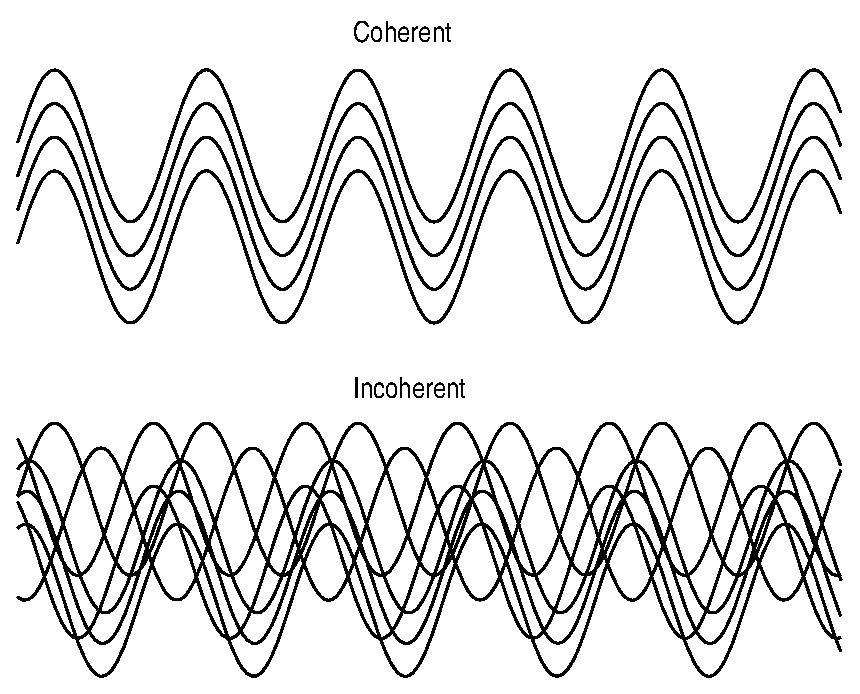
\includegraphics[width=0.7\textwidth]{coherent-vs-incoherent.eps}
	\caption{Coherent v.s. incoherent light}
	\label{fig:coherent-vs-incoherent.eps}
\end{figure}

The coherence of light refers to the property of light waves where the phase relationship between the waves is consistent over time and space, corresponding to temporal and spatial coherence:
\begin{itemize}
  \item \textbf{Temporal coherence:} Temporal coherence describes the correlation between the phases of a light wave at different points along its propagation direction. It indicates how monochromatic (i.e. single-frequency) a light source is.
  \item \textbf{Spatial coherence:} Spatial coherence describes the correlation between the phases of a light wave at different points across the wavefront, perpendicular to the direction of propagation. It indicates the uniformity of the phase across the wavefront, as illustrated in \cref{fig:coherent-vs-incoherent.eps}. High spatial coherence means that the light waves across different points on the wavefront are in phase.
\end{itemize}

\begin{figure}[H]
	\centering
	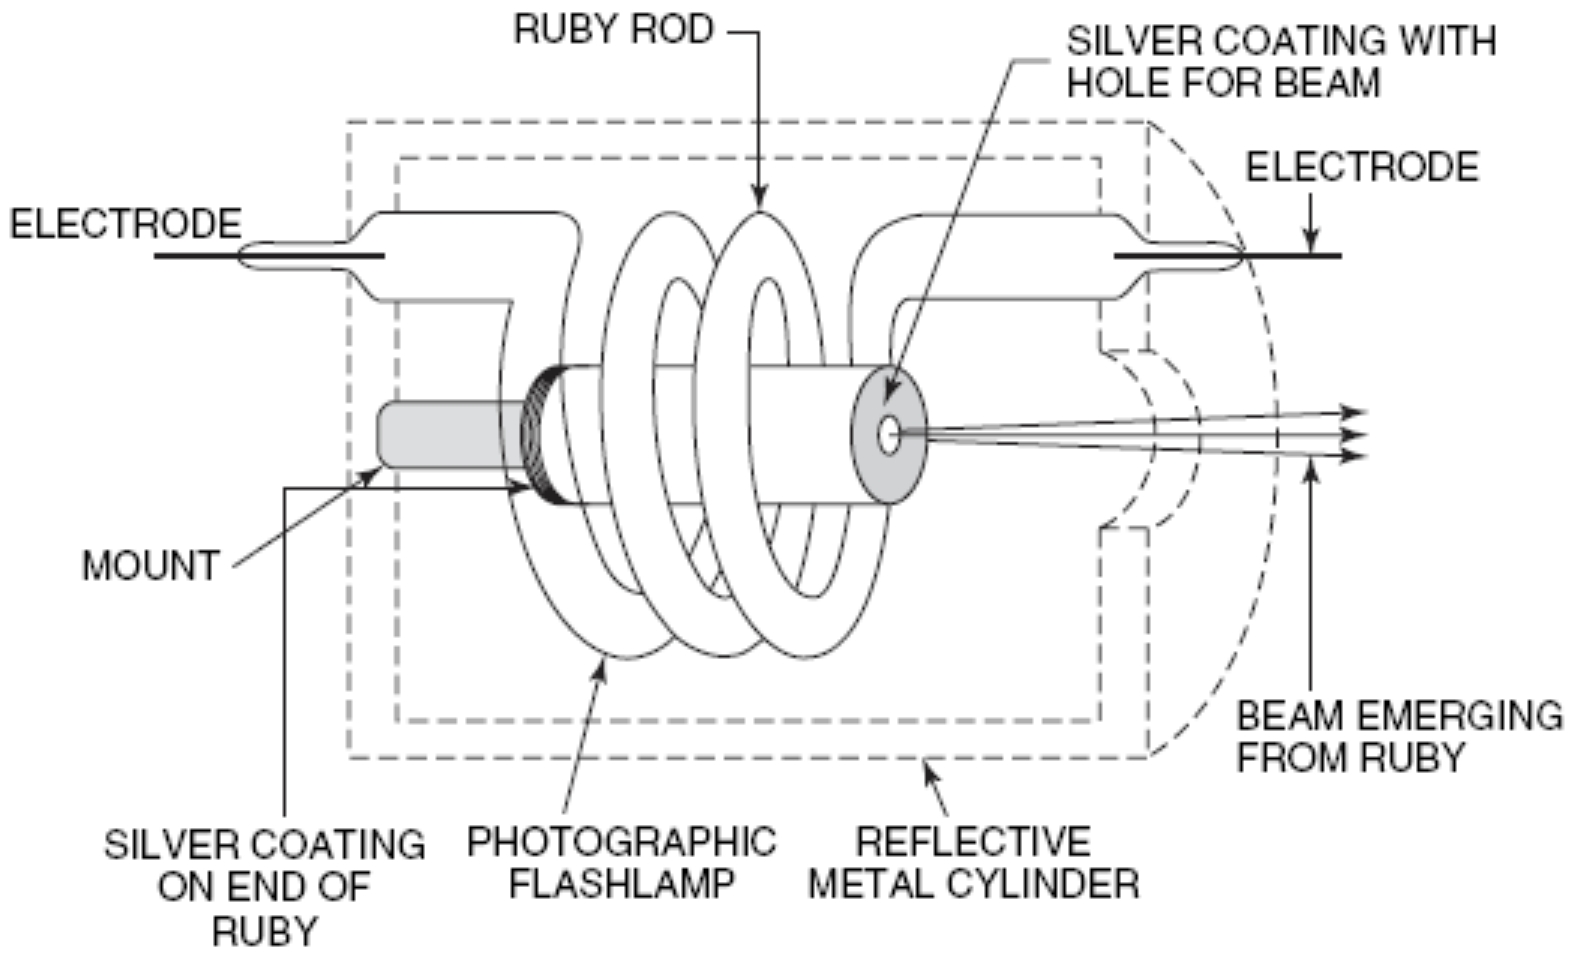
\includegraphics[width=0.9\textwidth]{first_laser.jpg}
	\caption{Structure of the first laser \cite{Hecht2008}}
	\label{fig:first_laser}
\end{figure}

The most common coherent visible light source is Laser, which stands for \textit{\textbf{L}ight \textbf{A}mplification by the \textbf{S}timulated \textbf{E}mission of \textbf{R}adiation}. It was first invented by Theodore Maiman in 1959, with the structure shown in \cref{fig:first_laser} \cite{Hecht2008, Gordon1959, Cartlidge2007}. It differs from other sources of light in that it emits coherent light, which is suitable for holographic projection. However, the coherent and monochromatic property of laser also has a side effect of speckle noise in the reconstructed image \cite{John1966}, which is one of the major problems affecting the image quality of holographic projections and has seen lots of efforts to cope with it in the literature \cite{Cable2004,Stangner2017,Deng2021,Hands2022}.


\subsection{Diffraction} \label{sec:Diffraction}

This section delves into how light interacts with apertures, leading to diffractions. Understanding diffraction is essential for holography, as it explains how light can be manipulated to reconstruct three-dimensional light fields. The principles of diffraction and interference underpin the essential process of holographic projection, making it possible to accurately recreate complex wavefronts and achieve true 3D visualization.

\begin{figure}[H]
  \centering
  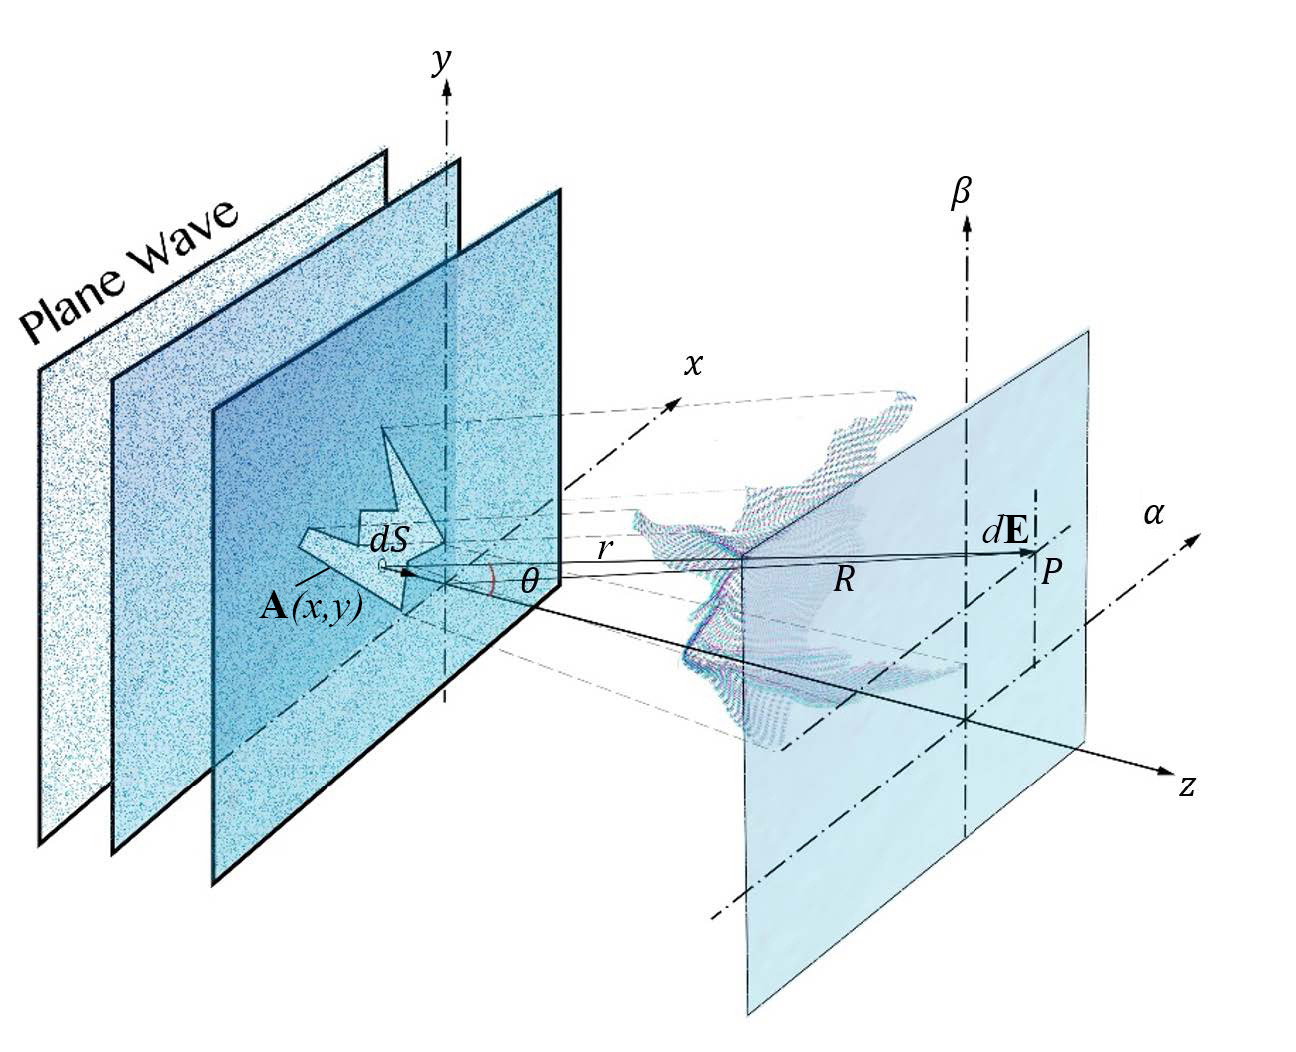
\includegraphics[width=0.8\textwidth]{diffraction_coordinate_definition.jpg}
  \caption{Diffraction geometry}\label{fig:diffraction_coordinate_definition}
\end{figure}

To model how light diffracts through a 2D aperture, we first set up a coordinate system as shown in \cref{fig:diffraction_coordinate_definition}, where the aperture is denoted by $A(x, y)$ and the diffracted field is denoted by $E(\alpha, \beta, z)$. $R$ defines the distance between point $P$ and the origin of the aperture ($(x,y)=(0,0)$), $r$ defines the distance between point $P$ and a point on the aperture, and $\theta$ defines the angle $r$ from the $z$-axis. Then by trigonometry we can have the following identities:
\begin{align}
  cos(\theta) & = \frac{z}{r}                      \label{eq:trignometry-theta} \\
  R^2         & = \alpha ^2 + \beta ^2 + z^2       \label{eq:trignometry-R} \\
  r^2         & = (\alpha-x)^2 + (\beta-y)^2 + z^2 \label{eq:trignometry-r}
\end{align}

\begin{figure}[H]
  \centering
  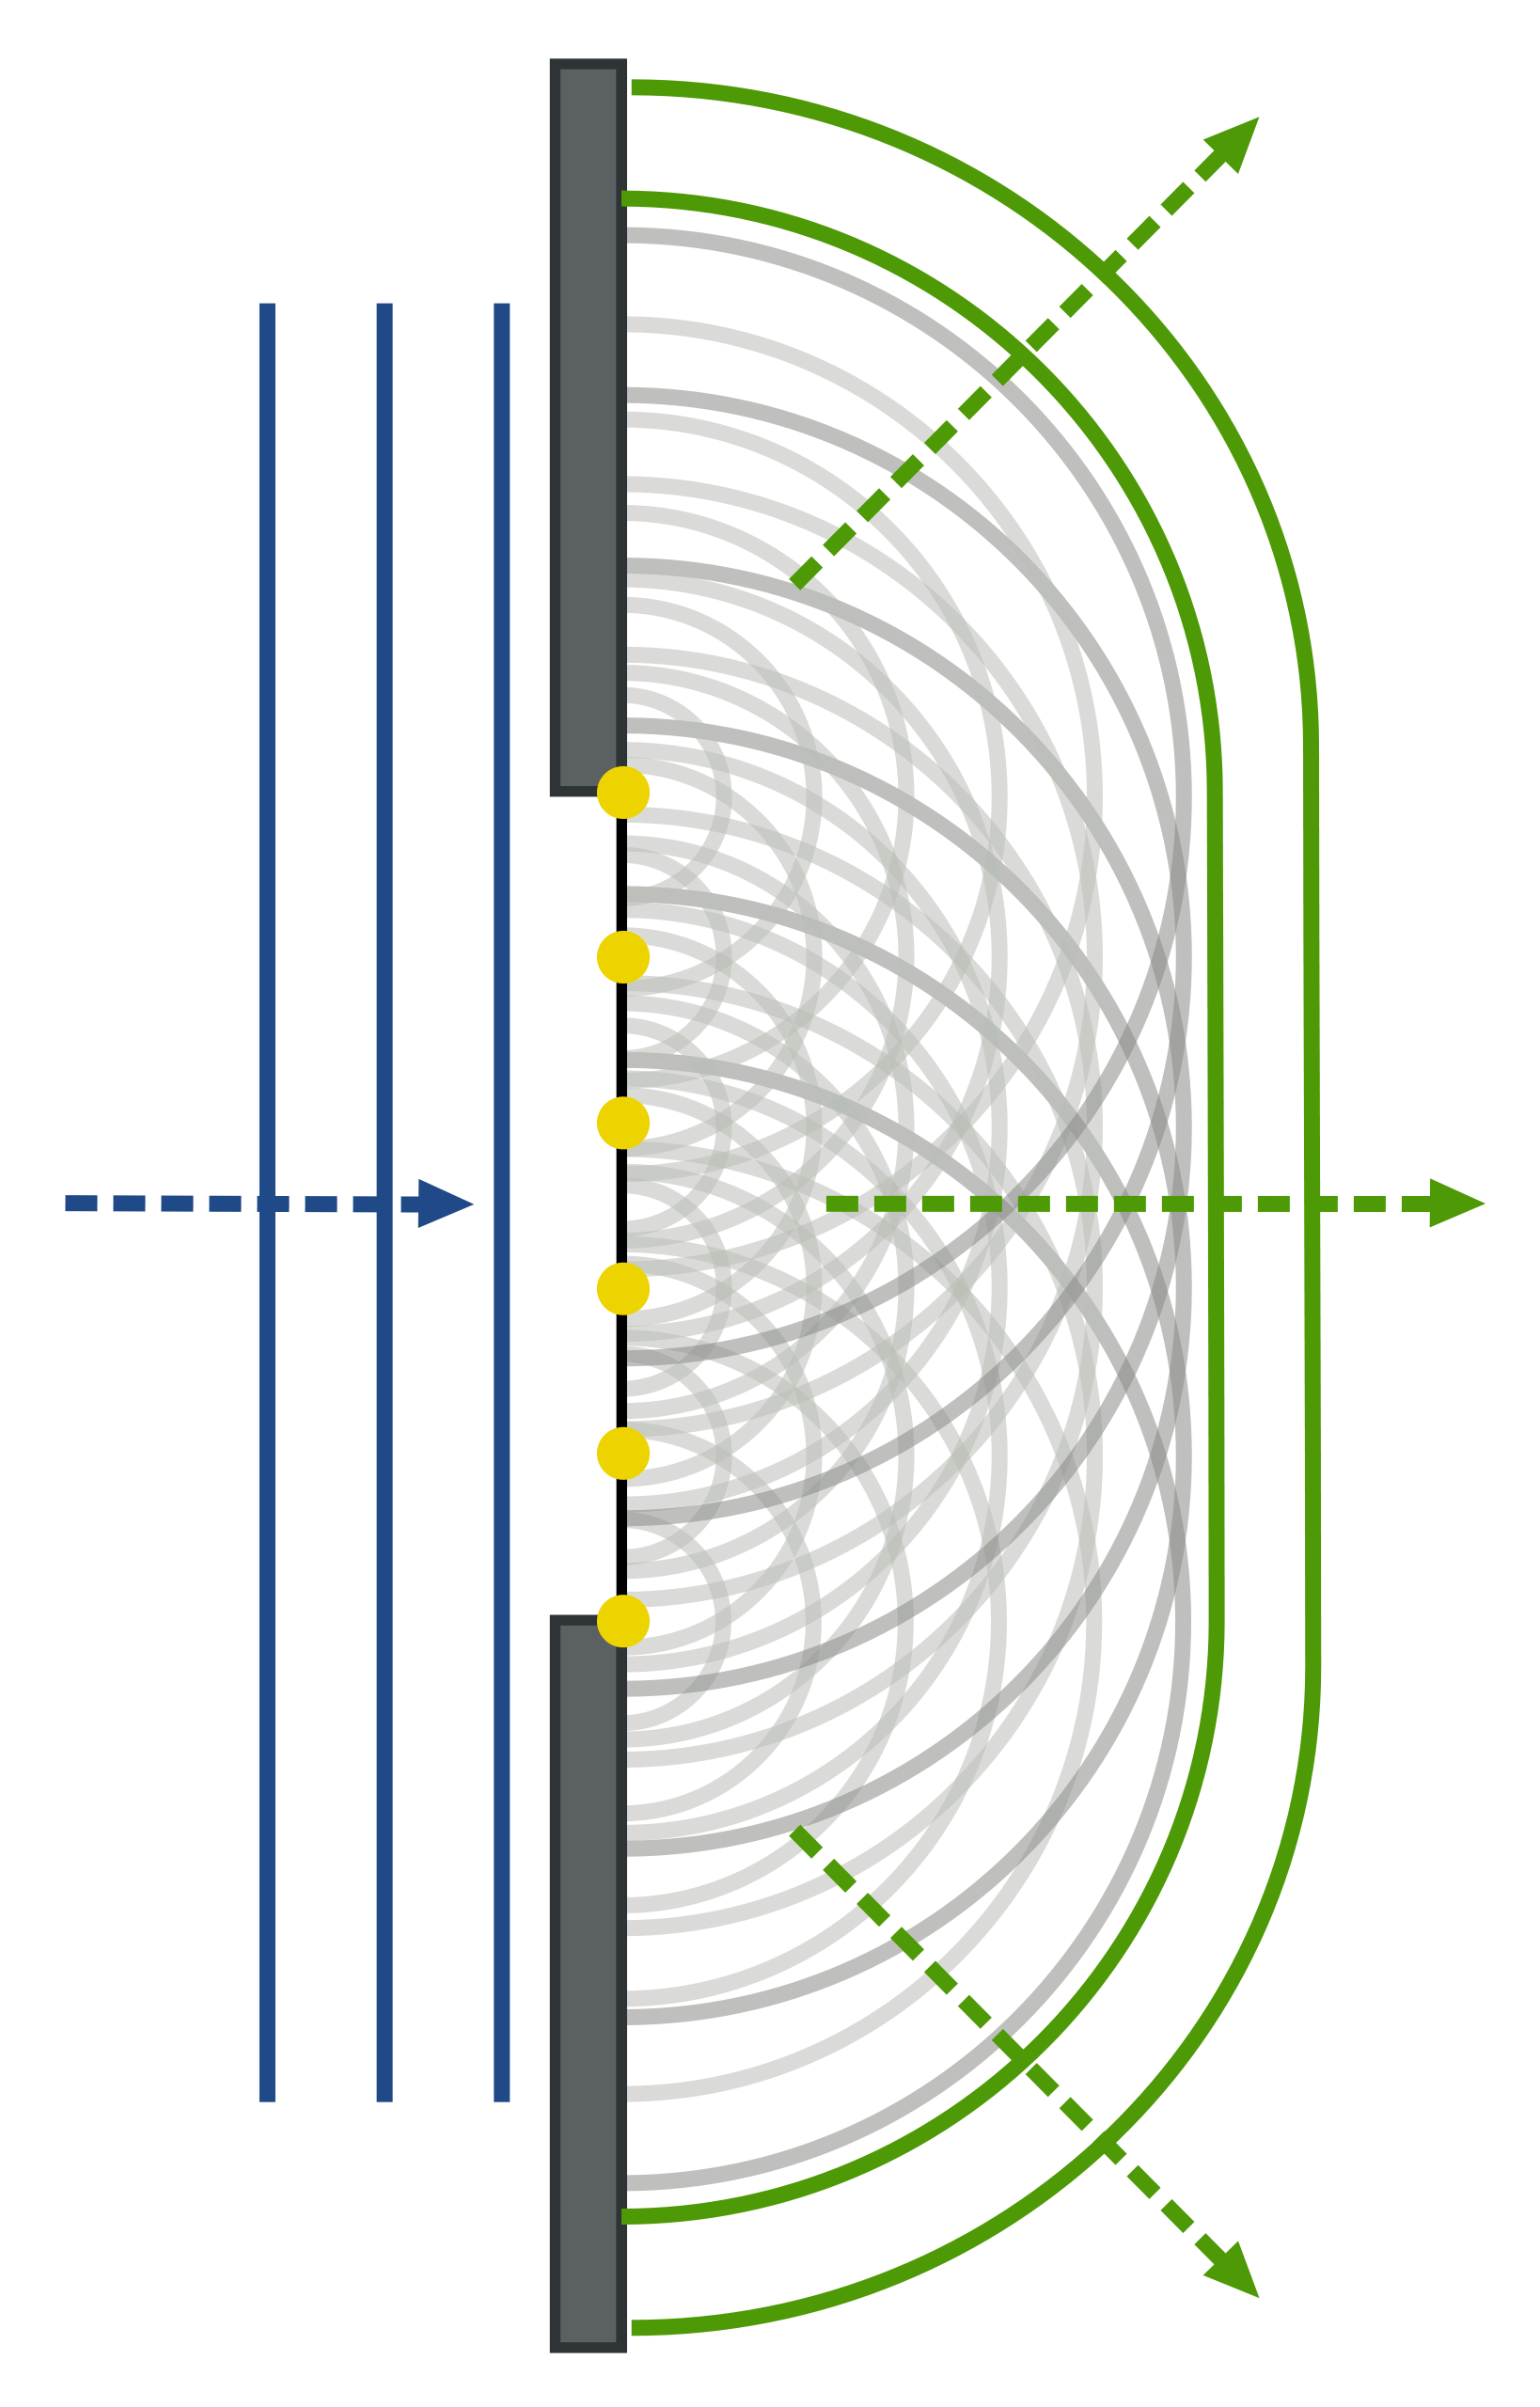
\includegraphics[width=0.3\textwidth]{huygens_wavelets_principle.png}
  \caption{Huygens-Fresnel wavelet principle \cite{Nordmann2007}}\label{fig:huygens_wavelets_principle}
\end{figure}

The Huygens-Fresnel principle states that every point on a wavefront is itself the source of outgoing secondary spherical wavelets, which can be expressed mathematically as follows when $r\gg \lambda$ \cite{Goodman2017}:
\begin{equation}
  E(\alpha, \beta, z) = \frac{1}{j\lambda} \iint A(x,y)\frac{e^{jkr}}{r} cos(\theta) dxdy \label{eq:huygens-fresnel-principle}
\end{equation}

Applying the identities in \cref{eq:trignometry-theta} - \cref{eq:trignometry-r},  \cref{eq:huygens-fresnel-principle} becomes:
\begin{align}
  E(\alpha, \beta, z) & = \frac{z}{j\lambda} \iint A(x,y)\frac{e^{jkr}}{r^2} dxdy                    \label{eq:huygens-fresnel-principle-substituded-cos}                                                      \\
                      & = \frac{z}{j\lambda} \iint A(x,y)\frac{e^{jk\sqrt{(\alpha-x)^2 + (\beta-y)^2 + z^2}}}{(\alpha-x)^2 + (\beta-y)^2 + z^2} dxdy \label{eq:huygens-fresnel-principle-substituded-r-square}
\end{align}

Unfortunately, \cref{eq:huygens-fresnel-principle-substituded-r-square} cannot be solved analytically except for few specific aperture functions $A(x,y)$, so we have to make some approximations in order to solve for arbitrary $A(x,y)$, the common methods are \textit{Fresnel} and \textit{Fraunhofer} approximations for regions depicted in \cref{fig:fresnel_fraunhofer_approximations}.

\begin{figure}[H]
  \centering
  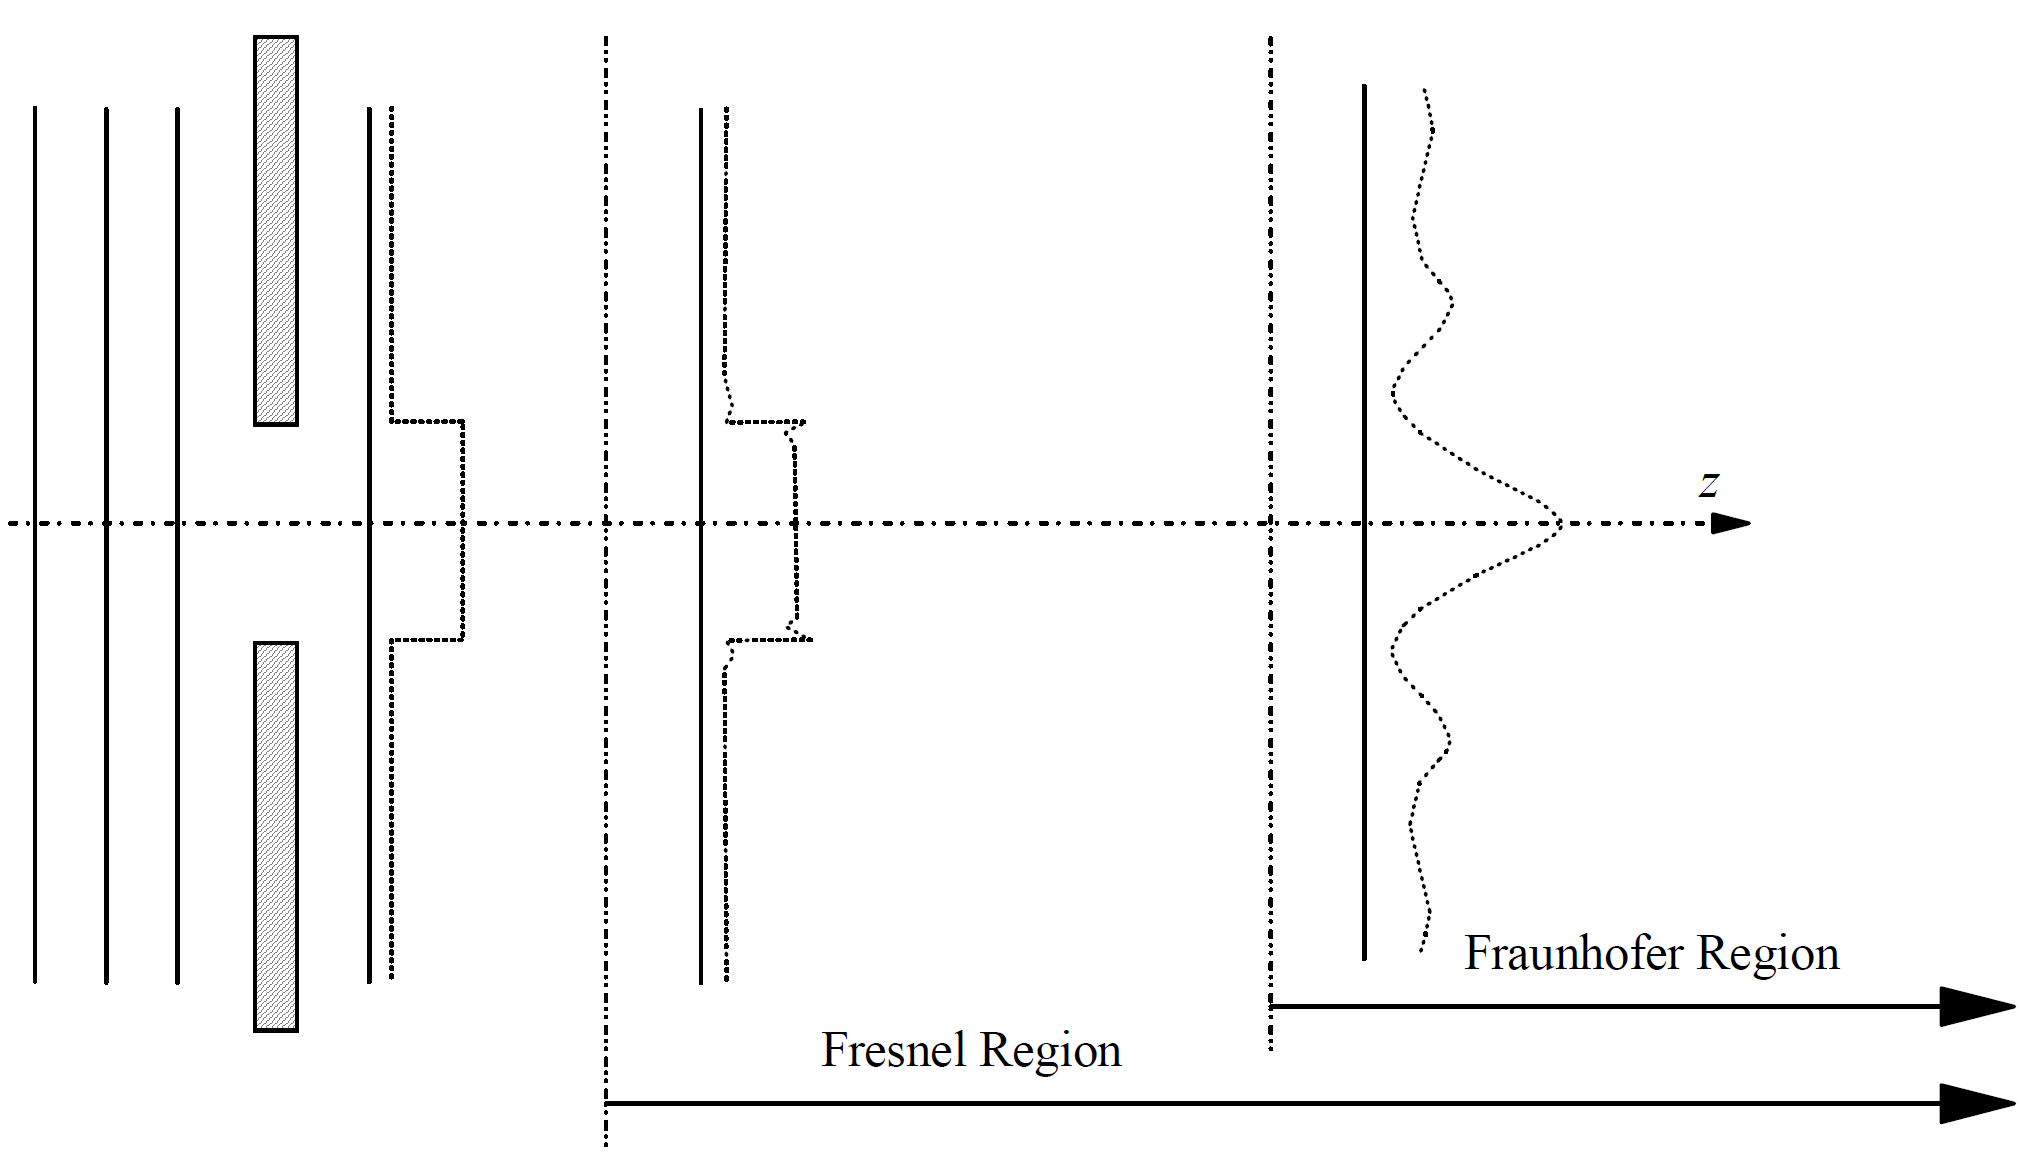
\includegraphics[width=0.9\textwidth]{fresnel_fraunhofer_approximations.png}
  \caption{Fresnel and Fraunhofer region \cite{Wilkinson2019}}\label{fig:fresnel_fraunhofer_approximations}
\end{figure}


\subsubsection{Fresnel Approximation}
\begin{equation}
  \sqrt{1+d} = 1 + \frac{1}{2}d - \frac{1}{8}d^2 + \cdots \label{eq:binomial-expension}
\end{equation}
Fresnel approximation replaces expressions for spherical waves by quadratic-phase exponentials, using the binomial expansion of the square root (given in \cref{eq:binomial-expension}) to approximate $r$ in \cref{eq:huygens-fresnel-principle-substituded-cos} \cite{Goodman2017}.

Retaining only the first two terms of the expansion gives:
\begin{align}
  r & = \sqrt{(\alpha-x)^2 + (\beta-y)^2 + z^2}                                                                                                              \\
    & = z \sqrt{1 + \left( \frac{\alpha-x}{z} \right)^2 + \left(\frac{\beta-y}{z}\right)^2}                                                                  \\
    & \approx z \left[ 1 + \frac{1}{2} \left( \frac{\alpha-x}{z} \right)^2 + \frac{1}{2} \left(\frac{\beta-y}{z}\right)^2 \right] \label{eq:r-approximation}
\end{align}

For the $r^2$ in the denominator of \cref{eq:huygens-fresnel-principle-substituded-cos}, the error introduced by dropping all terms but $z$ is generally acceptably small (i.e. $r^2\approx z^2$), and for the $r$ appearing in the exponent in the numerator of \cref{eq:huygens-fresnel-principle-substituded-cos}, errors are much more critical \cite{Goodman2017}. So, by substituting \cref{eq:r-approximation} for the $r$ in the numerator of \cref{eq:huygens-fresnel-principle-substituded-cos} and substituting $z$ for the $r$ in the denominator, we have:
\begin{align}
  E(\alpha, \beta, z) & \approx \frac{z}{j\lambda} \iint A(x,y)\frac{e^{jkz \left[ 1 + \frac{1}{2} \left( \frac{\alpha-x}{z} \right)^2 + \frac{1}{2} \left(\frac{\beta-y}{z}\right)^2 \right]}}{z^2} dxdy \\
                      & = \frac{e^{jkz}}{j\lambda z} e^{j\frac{k}{2z}(\alpha^2+\beta^2)} \iint \left\{A(x,y)e^{j\frac{k}{2z}(x^2+y^2)}\right\}e^{-j\frac{2\pi}{\lambda z}(\alpha x+\beta y)}dxdy    \\
                      & = \frac{e^{jkz}}{j\lambda z} e^{j\frac{k}{2z}(\alpha^2+\beta^2)} \mathcal{F} \left\{A(x,y)e^{j\frac{k}{2z}(x^2+y^2)}\right\}
\end{align}
where $\mathcal{F}$ denotes the Fourier Transform, implemented on computers using the Fast Fourier Transform (FFT) function. Such method of including Fourier Transform (FT) in the study of optics is also named `Fourier Optics'.

Now we have a more simple and solvable expression than \cref{eq:huygens-fresnel-principle-substituded-r-square}. And also, as we are only interested in the scaling of relative points at $P$ with respect to each other, so it is safe to normalise the multiplier term before the Fourier Transform to 1 \cite{Wilkinson2019}. So we can express the diffraction pattern in Fresnel region as:
\begin{equation}
  E_{Fresnel\ region}(\alpha, \beta, z) = \mathcal{F} \left\{A(x,y)e^{j\frac{k}{2z}(x^2+y^2)}\right\}
  \label{eq:fresnel-diffraction}
\end{equation}


\subsubsection{Fraunhofer Approximation}
Fraunhofer diffraction is a form of diffraction in which the distance between the light source and the receiving screen are in effect at infinite, so that the wave fronts can be treated as planar rather than spherical \cite{Daintith2009}. Fraunhofer approximation is very stringent, it assumes that the distance between the light source and the receiving screen are in effect at infinite:
\begin{equation}
  z\gg \frac{k(x^2+y^2)_{max}}{2}
\end{equation}

so that the wave fronts can be treated as planar rather than spherical \cite{Daintith2009}, then the $e^{j\frac{k}{2z}(x^2+y^2)}$ term tends to $1$, and \cref{eq:fresnel-diffraction} becomes:
\begin{equation}
  E_{Fraunhofer\ region}(\alpha, \beta) = \mathcal{F} \left\{A(x,y)\right\}
  \label{eq:fraunhofer-diffraction}
\end{equation}

which suggests that the far field pattern is simply the Fourier Transform of the aperture function.


\subsection{Spatial Light Modulator (SLM)} \label{sec:SLM}
SLMs are critical components in computer-generated holography (CGH). An SLM is a device used to control the amplitude or phase of light waves in a spatially varying manner. SLMs typically consist of a two-dimensional (2D) array of pixels, each of which can modulate the light either passing through or reflected from it. These pixels are usually addressed by electronic signals, allowing precise manipulation of the light wavefront. The modulation can be achieved through various mechanisms, such as liquid crystal (LC) SLMs, magneto-optic SLMs, deformable mirror SLMs, multiple-quantum-well SLMs, or acousto-optic Bragg cells \cite{Goodman2017}.

\begin{figure}[H]
  \centering
  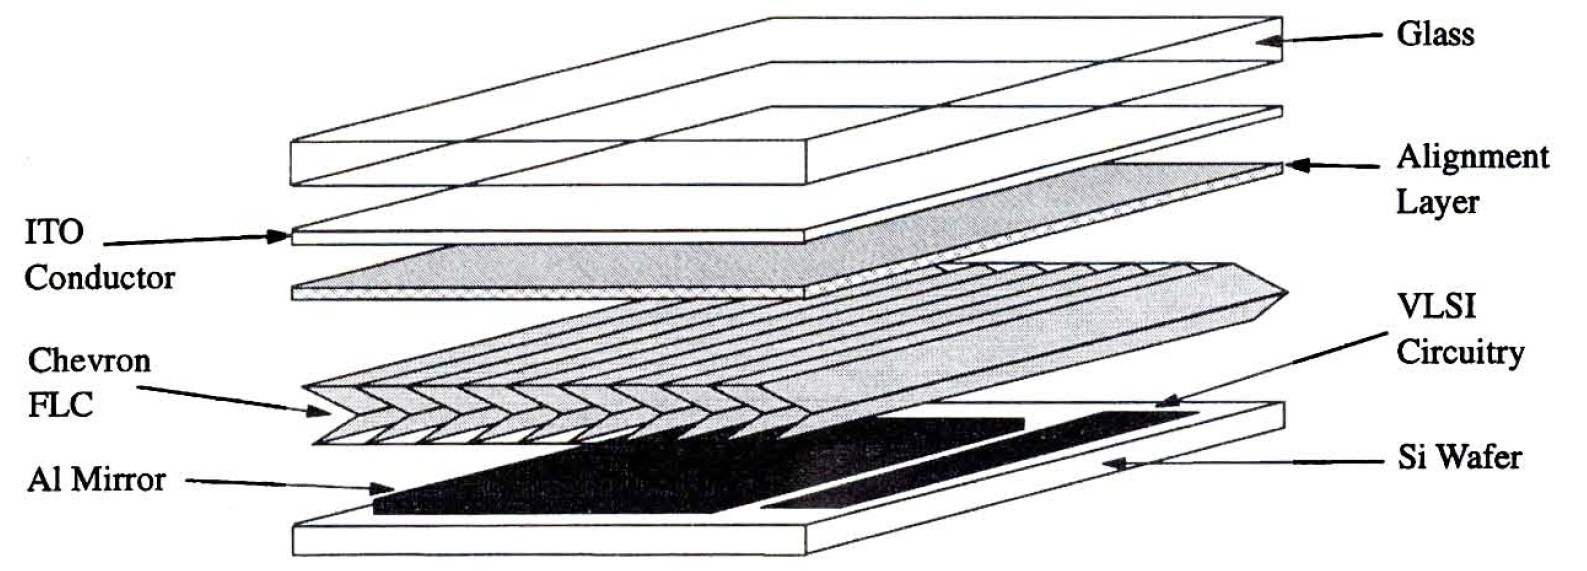
\includegraphics[width=1.0\textwidth]{SLM_pixel_structure.jpg}
  \caption{A single FLC backplane SLM pixel structure \cite{Wilkinson1994}} \label{fig:SLM_pixel_structure}
\end{figure}

The typical structure of a Ferroelectric Liquid Crystal (FLC) SLM pixel is shown in \cref{fig:SLM_pixel_structure}. The horizontal dimension of a single pixel, which is called the pixel pitch, is on scale of a few \SI{}{\micro\metre}. LCs are anisotropic materials, which have different refraction index in different axis. And the modulation is achieved by controlling the tilt of the angle of the LCs. For the FLCs, the tilt angle is controlled by the electric field across them. Therefore the FLCs are sandwiched between the Indium Tin Oxide (ITO) conductor and the aluminium (Al) mirror, aside which is a Very Large Scale Integration (VLSI) circuitry to control the voltage and the electric field across the FLCs, hence modulates the phase of the incident light. Aligning millions of pixels in a grid produces an SLM which can spatially modulate the wavefront of the incident light.
\begin{figure}[H]
  \centering
  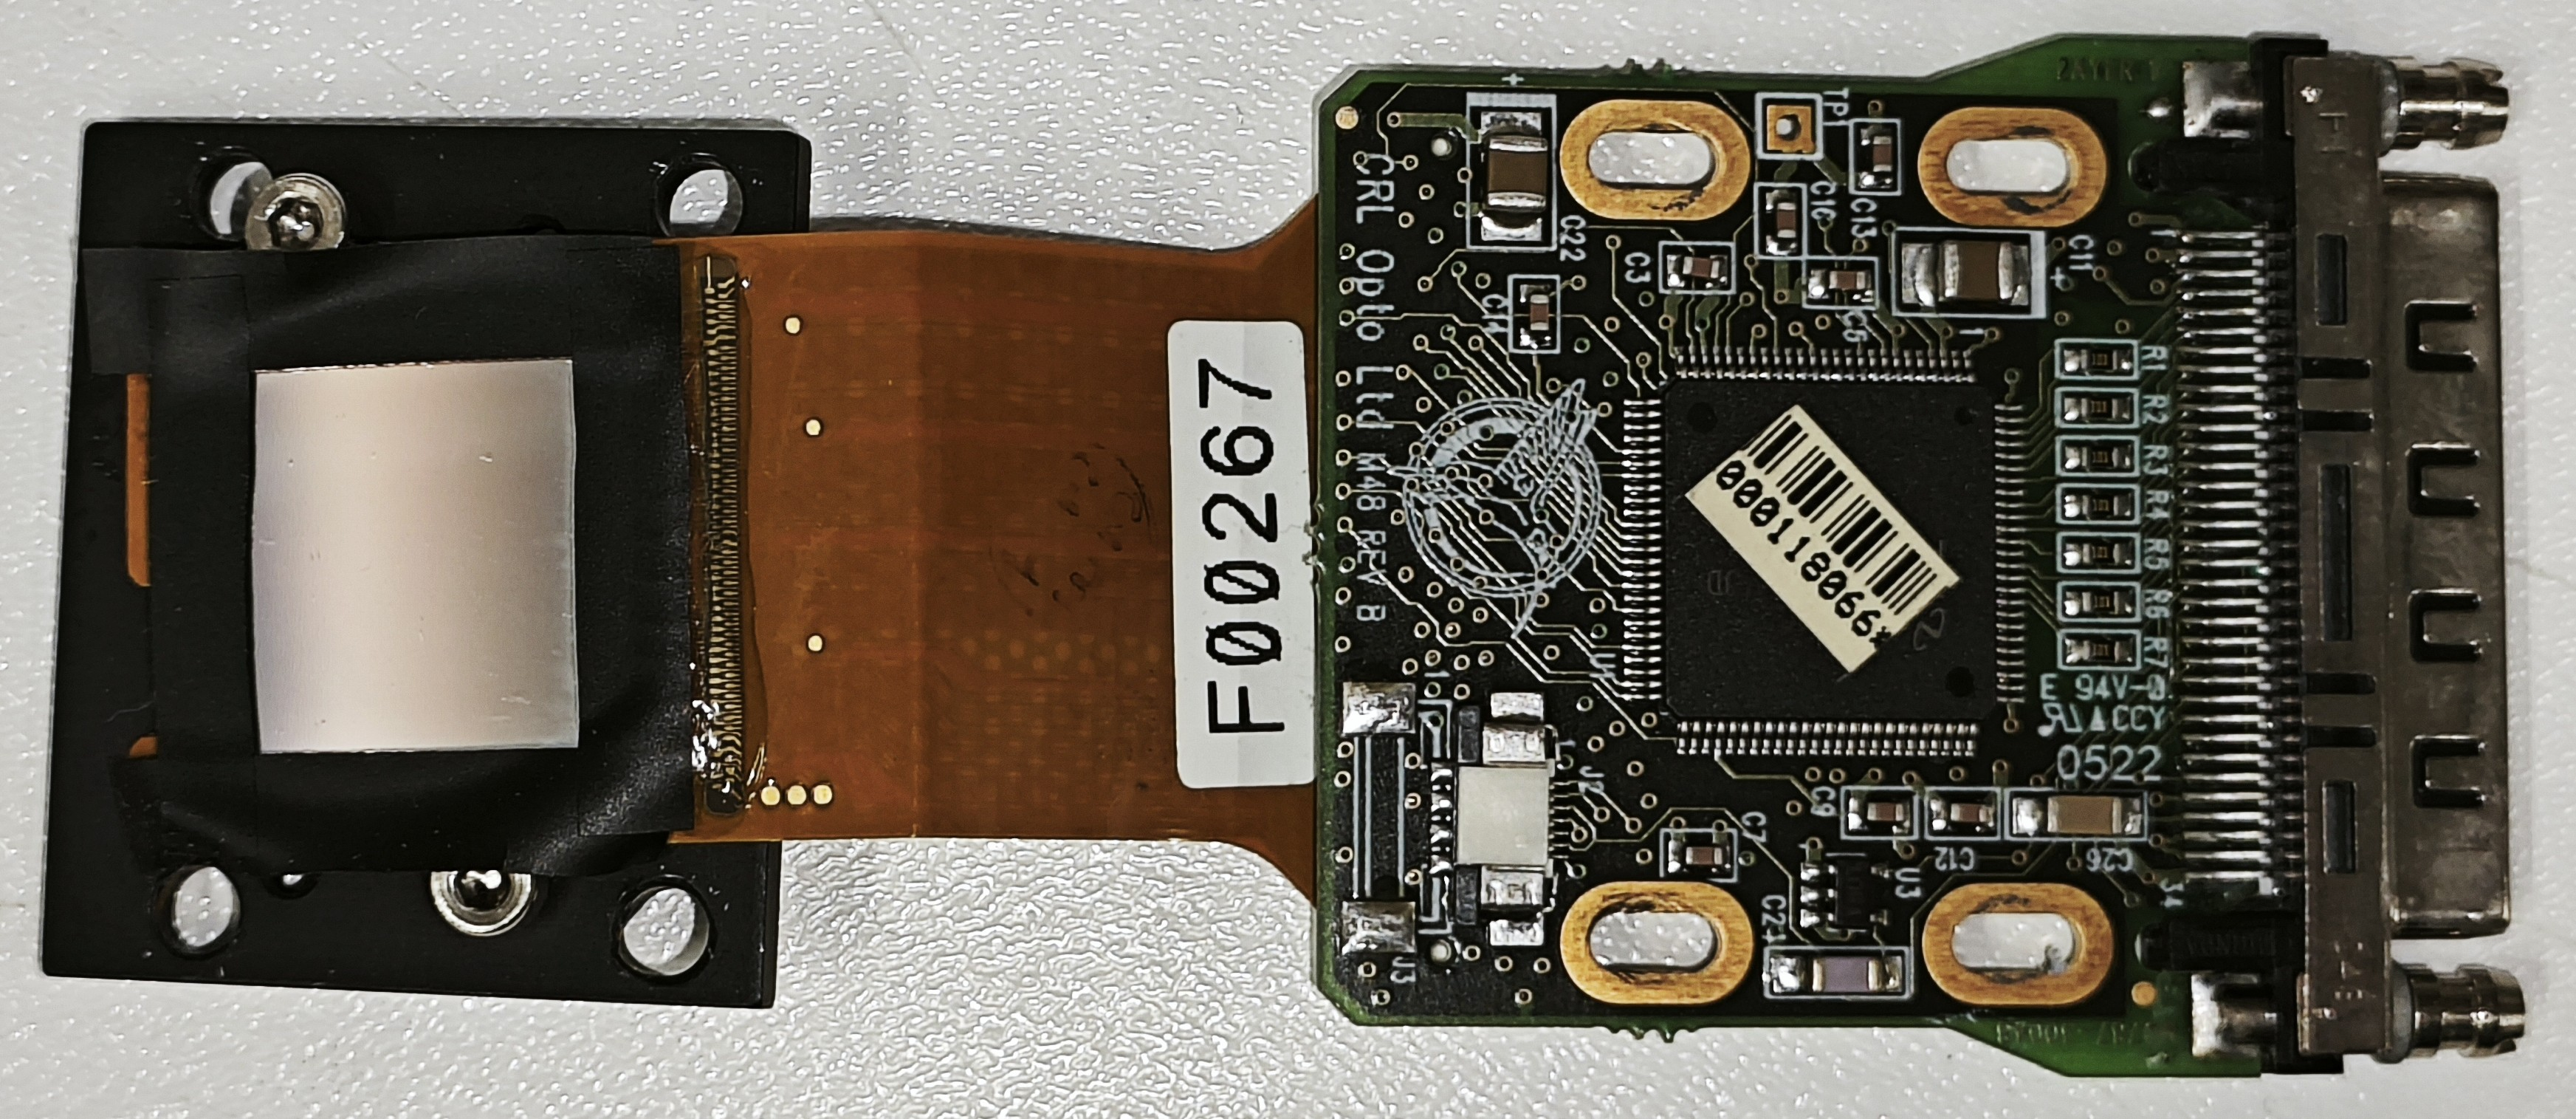
\includegraphics[width=0.7\textwidth]{SLMPhoto.jpg}
  \caption{Photo of an FLC SLM} \label{fig:SLMPhoto}
\end{figure}
A photo of an FLC SLM is shown in \cref{fig:SLMPhoto}. The SLM used in this research is a binary phase SXGA-R2 ForthDD FLC SLM with a refresh rate of 1440Hz, a pixel pitch of \SI{13.6}{\micro\metre} and a resolution of $1280px \times 1024px$.

\begin{figure}[H]
  \centering
  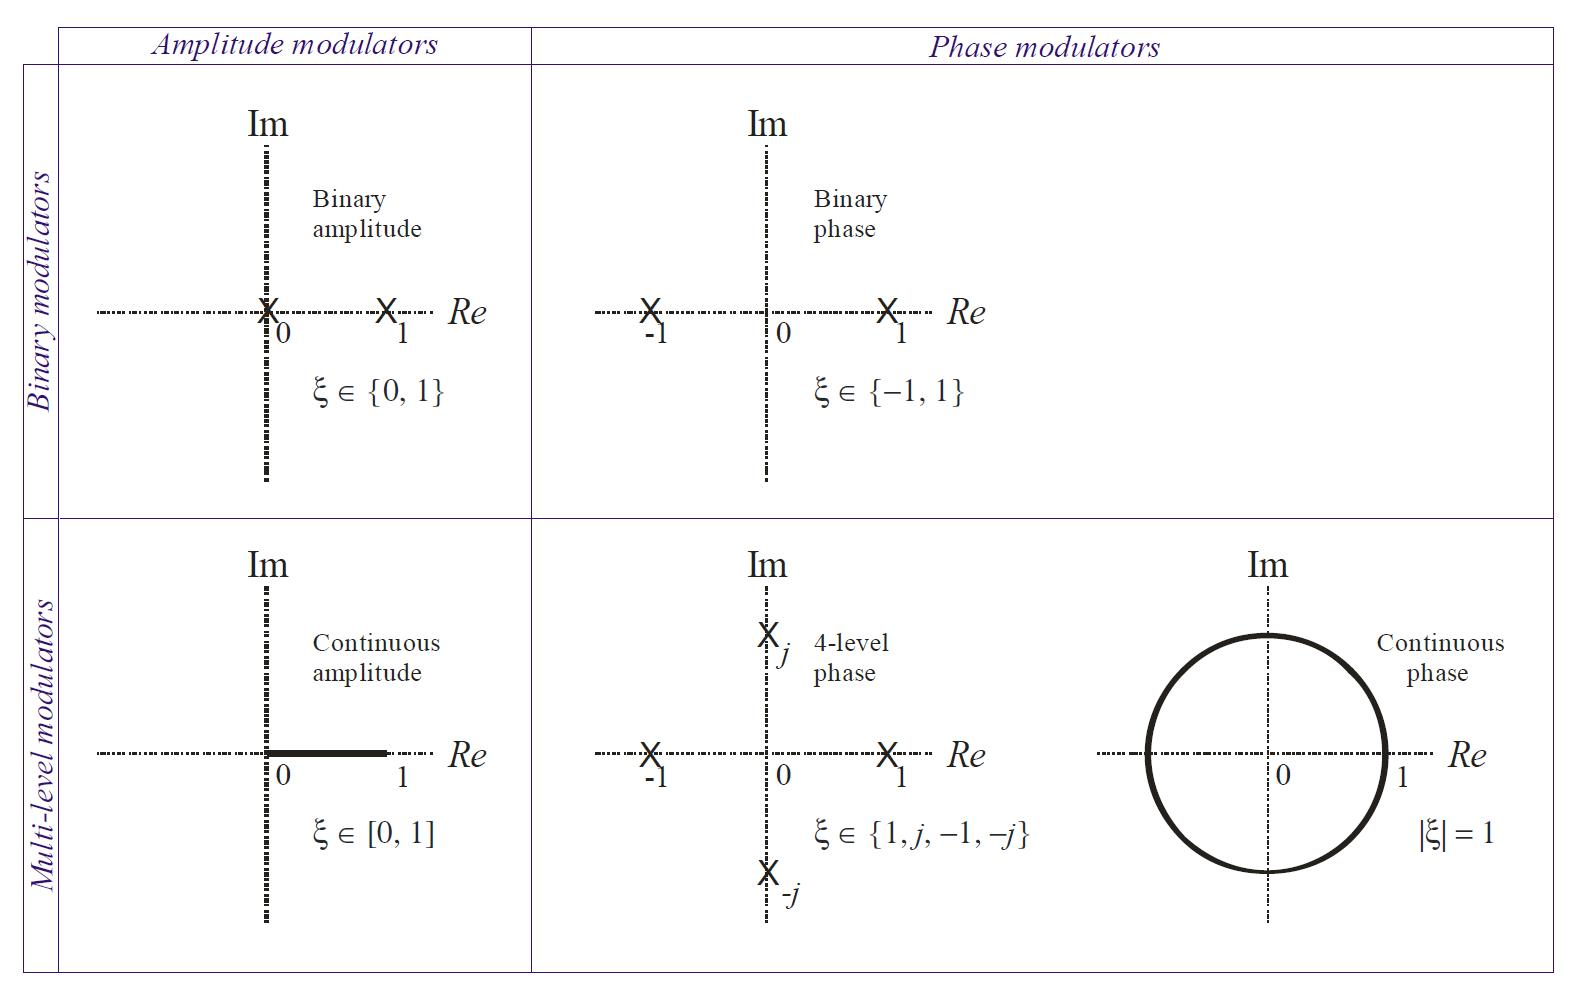
\includegraphics[width=1.0\textwidth]{modulation_loci.jpg}
  \caption{Modulation schemes of the SLMs \cite{Cable2006}} \label{fig:modulation_loci}
\end{figure}

Currently available SLMs have one of the four modulation schemes, as illustrated in \cref{fig:modulation_loci} \cite{Cable2006}, which are:

\begin{itemize}
  \item \textbf{Multi-level Amplitude} modulators can modulate each pixel from zero transmission (0) to full transmission (1), either continuously or in discrete steps. (e.g. nematic liquid crystal display \cite{Schadt1971}, found for example in laptops and many conventional video projectors)
  \item \textbf{Binary Amplitude} modulators can switch each pixel to zero transmission (0) or full transmission (1), but nothing in between. (e.g. deformable mirror device \cite{Pape1983}, ferroelectric liquid crystal display \cite{Johnson1993}, both used in high-end video projectors)
  \item \textbf{Multi-level Phase} modulators can modulate the phase shift imparted by each pixel from 0 to 2$\pi$ radians, either continuously or in discrete steps. (e.g. Nematic liquid crystal devices \cite{Lee2004})
  \item \textbf{Binary Phase} modulators can switch each pixel for a phase shift of either 0 or $\pi$ radians. (e.g. Ferroelectric liquid crystal displays \cite{Broomfield1992})
\end{itemize}

Among the four modulation schemes, phase modulations are of higher interest for the purpose of holography, because amplitude modulators, either multi-level or binary, block light at the SLM, causing waste of energy, leading to poorer energy efficiency. And also, amplitude modulation always has a zero-order (forming a central bright spot), because the average amplitude is always between 0 and 1; on the contrary, phase modulation can suppress the zero-order by designing the hologram to have zero average.

As there is no fully complex modulator available yet, we need algorithms to generate phase-only holograms, and such process is called phase retrieval. There are currently many algorithms for such purpose, which will be discussed in \cref{sec:cgh}.

\subsubsection{Rotational symmetries in the binary phase modulation} \label{sec:Rotational symmetries in the binary phase modulation}

The spatial light modulator (SLM) used in this thesis is a binary phase modulator. As the binary phase modulation is purely real (i.e. it's only switching between $0^\circ$ and $180^\circ$, corresponding to 1 and -1 values of $A^*(x,y)$), the complex conjugate $A^*(x,y)$ is the same as $A(x,y)$:
\begin{equation} \label{eq:AequalsAstar}
  A^*(x,y) = A(x,y)
\end{equation}
because the Fourier transform of $A^*(x,y)$ is the same as the Fourier transform of $A(x,y)$
\begin{equation} \label{eq:AAstar}
  E(-\alpha, -\beta)=\mathcal{F}[A^*(x,y)]=\mathcal{F}[A(x,y)]=E(\alpha, \beta)
\end{equation}
So, at the Fraunhofer region, there is no distinction between the desired image and its $180^\circ$ rotation in the replay field, causing a symmetrical conjugate image rotated $180^\circ$ from the target image.

\begin{figure}[H]
  \centering
  \begin{subfigure}[t]{0.45\textwidth}
    \centering
    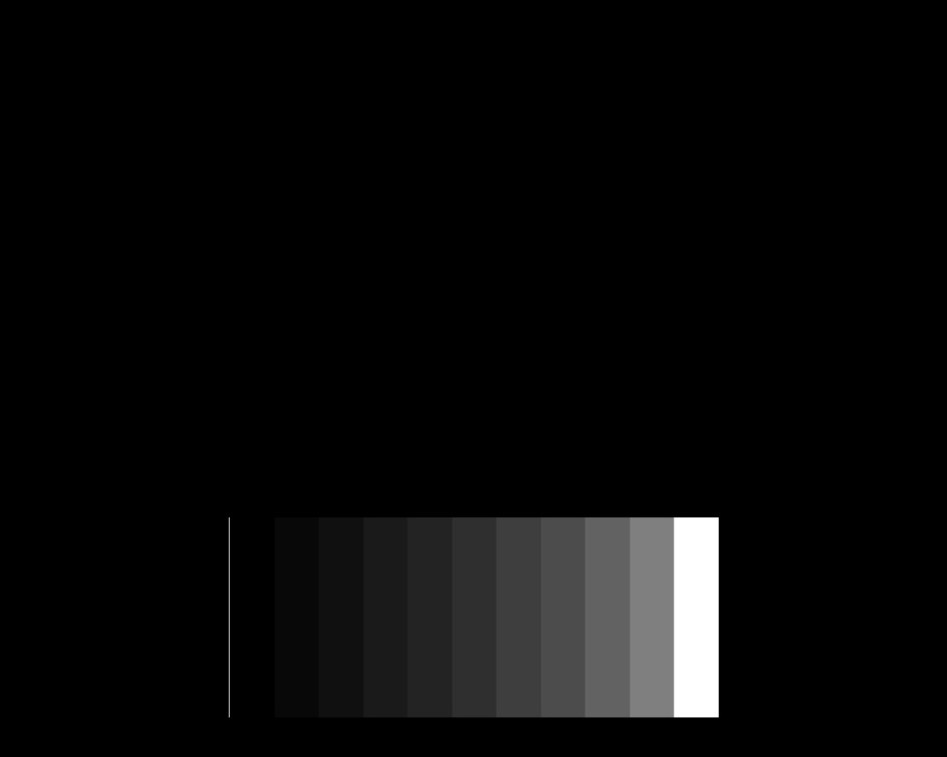
\includegraphics[width=\textwidth]{10_step_target.jpg}
    \caption{Target image}
    \label{fig:10_step_target}
  \end{subfigure}
  \hfill
  \begin{subfigure}[t]{0.45\textwidth}
    \centering
    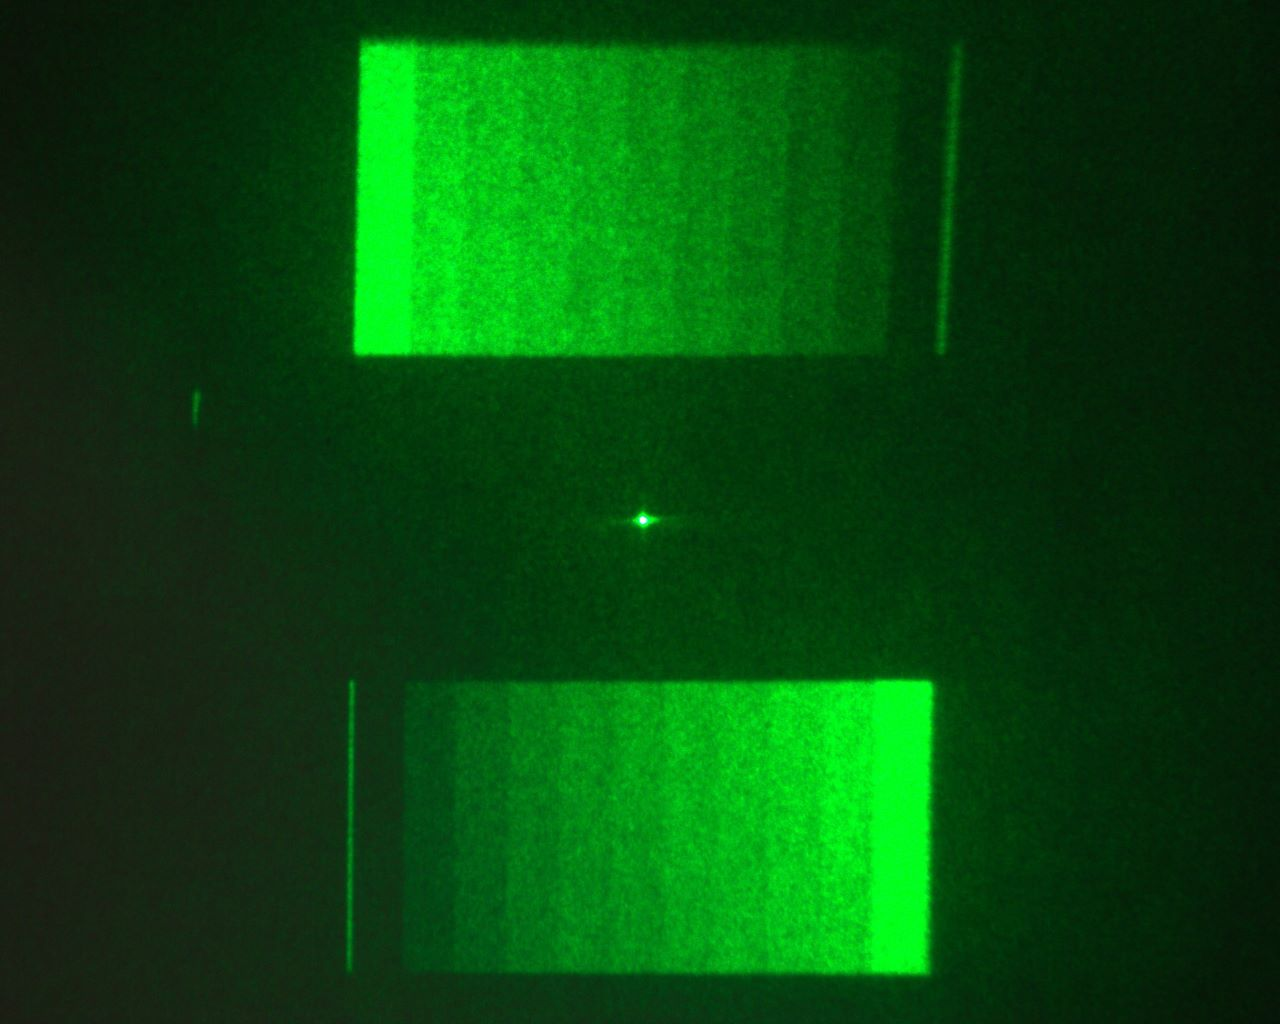
\includegraphics[width=\textwidth]{binary_phase_SLM_symmetry.jpg}
    \caption{Projection result}
    \label{fig:binary_phase_SLM_symmetry}
  \end{subfigure}

  \caption{Rotational symmetry in the projection result using the binary phase SLM}
  \label{fig:Rotational symmetry Binary SLM}
\end{figure}

To demonstrate such phenomena, the example target image shown in \cref{fig:10_step_target} generated the binary-phase hologram using the algorithm called one-step phase-retrieval (OSPR), which will be explained in detail in \cref{sec:One Step Phase Retrieval (OSPR) Algorithm}, and the projection output is shown in \cref{fig:binary_phase_SLM_symmetry}. The simplest workaround for this issue is to use only half of the reconstruction field, like the target image in \cref{fig:10_step_target}. However, the side effect of this is that half of the energy will be wasted, leading to higher power consumption and heat dissipation.



\newpage
\section{Computer-Generated Holography (CGH)}\label{sec:cgh}
Different from the traditional analogue optical holography and digital holography which both need a physically existing object to record the hologram, the CGH is a method to use computer algorithms to generate holograms without the need for the physical target object. Ideally, holograms can be simply computed using the inverse Fourier Transform, using the inverse functions of \cref{eq:fresnel-diffraction} and \cref{eq:fraunhofer-diffraction} derived in \cref{sec:Diffraction}. The inverse Fourier Transforms on most targets will end up with results in complex numbers; however, as mentioned in \cref{sec:SLM}, currently available SLMs cannot achieve fully complex modulation yet. Therefore, computer algorithms are needed to compute either phase-only or amplitude-only holograms, among which the former is preferred, as explained in \cref{sec:SLM}.

This section reviews the existing methods in the literature for calculating phase-only holograms. The phase hologram is labelled as $H$, so that it differs from the previous notation of $A$ for complex-valued hologram apertures. And the propagation function is unified as $\mathcal{P}$, which can be either the Fraunhofer propagation equation in \cref{eq:fresnel-diffraction} or the Fresnel propagation equation in \cref{eq:fraunhofer-diffraction} depending on the distance of the target field. Lastly, $R$ denotes the reconstruction intensity of the hologram (i.e. $R = \vert \mathcal{P}[e^{jH}] \vert ^2 $).

\begin{figure}[H]
  \centering
  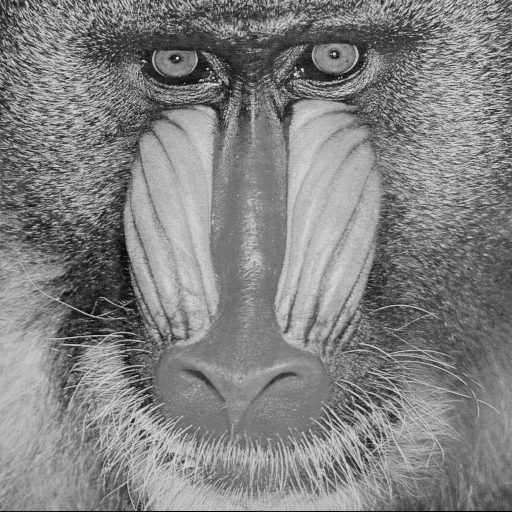
\includegraphics[width=0.3\textwidth]{mandrill.png}
  \caption{Sample target image of a mandrill ($T$) \cite{MANDRILL_REF}}\label{fig:mandrill.png}
\end{figure}

A sample image of a mandrill (shown in \cref{fig:mandrill.png}) is chosen from the University of Southern California Signal and Image Processing Institute (USC-SIPI) Image Database \cite{MANDRILL_REF} to test and compare the classical phase retrieval algorithms in the literature. As the square of the amplitude, which is the intensity of light, is the only visible component with the human eye \cite{Huang2024}, the diffracted electric field amplitude ($\vert E \vert$) will be targeted to match the square root of $T$.

To quantitatively analyse the reconstruction quality, two metrics are used in this sections, which are the normalised mean squared error (NMSE) \cite{MSE_REF} and the structural similarity index (SSIM) \cite{Wang2004_SSIM}.

The NMSE is calculated using \cref{eq:NMSE}:
\begin{equation}
  NMSE(x,y) = \frac{\frac{1}{n} * \sum (x - y)^2}{\sum (x)^2}
  \label{eq:NMSE}
\end{equation}
where $x$ is the target, $y$ is the measured output and $n$ is the number of pixels in $x$ and $y$. As the NMSE quantifies the total error between the measured output and the target, lower NMSE value indicates better quality. Different from the NMSE which calculates the absolute errors, the SSIM is a perception-based metric that considers the structural similarity as perceived, defined in \cref{eq:SSIM}:
\begin{equation}
  SSIM(x,y) = \frac{(2\mu_x\mu_y + C_1) + (2 \sigma _{xy} + C_2)}{(\mu_x^2 + \mu_y^2+C_1) (\sigma_x^2 + \sigma_y^2+C_2)}
  \label{eq:SSIM}
\end{equation}
where $\mu_x$ and $\mu_y$ are the mean values of the pixels in $x$ and $y$ respectively, $\sigma_x^2$ and $\sigma_y^2$ are the variance, $\sigma _{xy}$ is the covariance of $x$ and $y$, $C_1 = (k_1 L)^2$ and $C_2 = (k_2 L)^2$, where $L$ is the dynamic range of the pixel values and $k_1 = 0.01$ and $k_2 = 0.03$ by default \cite{Wang2004_SSIM}. Higher SSIM indicates better reconstruction quality.


\subsection{Phase Unwrapping Method}\label{sec:Naive algorithm}
The simplest method to get a phase-only hologram $H$ is by directly extracting the phase of the reverse propagation from the target field, discarding the amplitude component (e.g. for Fraunhofer propagation, $H$ will simply be the phase of the inverse Fourier transform $\mathcal{F} ^{-1}$ of the target field). This method is named as the Phase Unwrapping method in this thesis as it directly unwraps the phases from the complex values. The pseudocode of the Phase Unwrapping method is shown in \cref{alg:Naive algorithm} below:
\begin{algorithm}[H]
  \caption{Phase Unwrapping method}\label{alg:Naive algorithm}
  \textbf{Input:} Target image $T$, Propagation function $\mathcal{P}$ (e.g. Fresnel or Fraunhofer propagation)\\
  \textbf{Output:} Phase hologram $H$ and its reconstruction intensity $R$
  \begin{algorithmic}
    \State $E \gets \sqrt{T}$
    \State $A \gets \mathcal{P}^{-1}[E]$
    \State $H \gets \angle A$
    \State $R \gets \vert \mathcal{P}[e^{jH}] \vert ^2 $
  \end{algorithmic}
\end{algorithm}
where $j = \sqrt{-1} $, the $\angle$ sign means phase unwrapping (i.e. taking arguments of the complex numbers element-wise in the matrix), and $e^{jH}$ converts the angles back to complex numbers. All exponentials, modulus and square-root operators are carried out in an element-wise manner, so that the dimensions of $T$, $A$, $H$, $R$ and $E$ are all the same.

The Phase Unwrapping method (described in \cref{alg:Naive algorithm}) was then implemented in MATLAB and run on the sample target image shown in \cref{fig:mandrill.png}, with the distance set to infinity (i.e. in the Fraunhofer region using the propagation formula \cref{eq:fraunhofer-diffraction}). The results are shown in \cref{fig:Naive algorithm output} below:

\begin{figure}[H]
  \centering
  \begin{subfigure}[t]{0.3\textwidth}
    \centering
    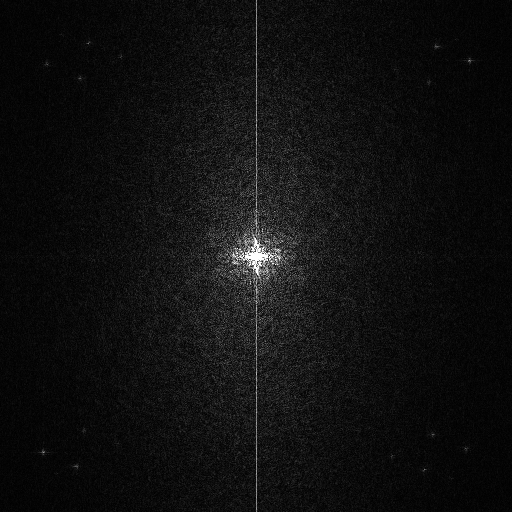
\includegraphics[width=\textwidth]{Naive_discarded_amplitude.png}
    \caption{Discarded amplitude ($\vert A\vert$)}
    \label{fig:Naive_discarded_amplitude}
  \end{subfigure}
  \hfill
  \begin{subfigure}[t]{0.3\textwidth}
    \centering
    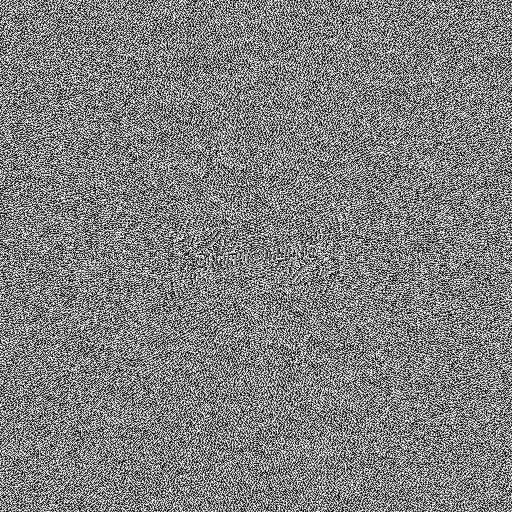
\includegraphics[width=\textwidth]{Naive_output_holo.png}
    \caption{Phase Hologram ($H$)}
    \label{fig:Naive_output_holo}
  \end{subfigure}
  \hfill
  \begin{subfigure}[t]{0.3\textwidth}
    \centering
    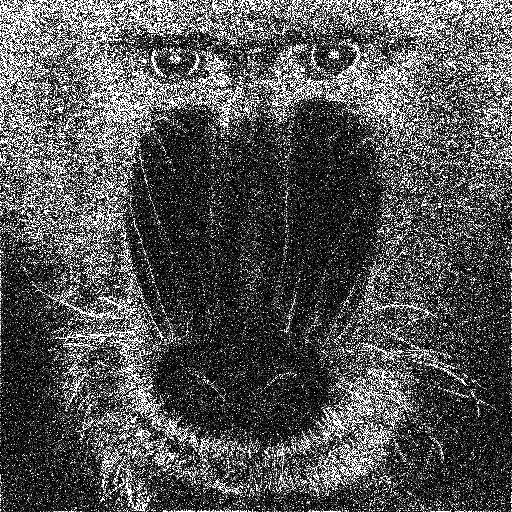
\includegraphics[width=\textwidth]{Naive_output_recon.png}
    \caption{Reconstruction ($R$)}
    \label{fig:Naive_output_recon}
  \end{subfigure}
  \caption{Phase Unwrapping method output}
  \label{fig:Naive algorithm output}
\end{figure}

After taking the inverse Fourier Transform, the amplitude and the phase of $A$ are shown in \cref{fig:Naive_discarded_amplitude} and \cref{fig:Naive_output_holo} respectively. The next step then discards the amplitude component (\cref{fig:Naive_discarded_amplitude}) and uses the phase component (in \cref{fig:Naive_output_holo}) as the phase hologram $H$. Then the phase hologram went through a forward propagation and the resulting reconstruction intensity is shown in \cref{fig:Naive algorithm output}.

The reconstruction intensity is very far from the desired target image in \cref{fig:mandrill.png}. It shows that, discarding amplitude has introduced a significant loss of information. From a signal processing point of view, the peak around the centre in \cref{fig:Naive_discarded_amplitude} corresponds to low spatial frequency signals, and discarding them causes the reconstruction in \cref{fig:Naive_output_recon} to lose low frequency components and effectively becomes an edge detector. Another explanation of the poor reconstruction quality is that, this method is assuming a uniform phase profile for the target image, which is physically difficult to achieve. A simple improvement can be made by adding a random phase to the target, as shown in the pseudocode below:

\begin{algorithm}[H]
  \caption{Improved Phase Unwrapping method with random phase added to the target field}\label{alg:Naive algorithm with random phase}
  \textbf{Input:} Target image $T$, Propagation function $\mathcal{P}$ (e.g. Fresnel or Fraunhofer propagation)\\
  \textbf{Output:} Phase hologram $H$ and its reconstruction intensity $R$
  \begin{algorithmic}
    \State $E \gets \sqrt{T} \times RandomPhase()$
    \State $A \gets \mathcal{P}^{-1}[E]$
    \State $H \gets \angle A$
    \State $R \gets \vert \mathcal{P}[e^{jH}] \vert ^2 $
  \end{algorithmic}
\end{algorithm}

The improved Phase Unwrapping method was implemented in MATLAB and produced the results in \cref{fig:Output of the improved Naive method} below:

\begin{figure}[H]
  \centering
  \begin{subfigure}[t]{0.3\textwidth}
    \centering
    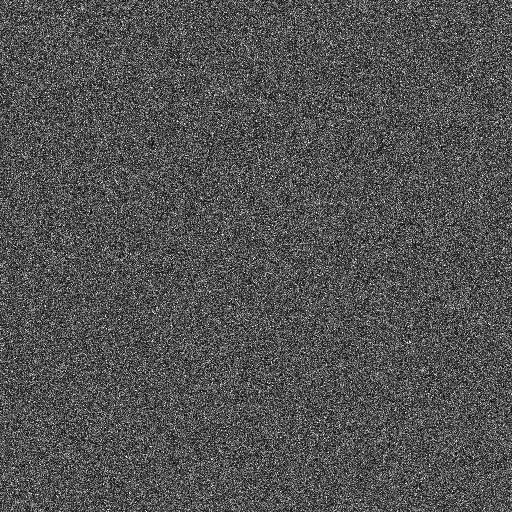
\includegraphics[width=\textwidth]{Naive_rand_discarded_amplitude.png}
    \caption{Discarded amplitude ($\vert A\vert$)}
    \label{fig:Naive_rand_discarded_amplitude}
  \end{subfigure}
  \hfill
  \begin{subfigure}[t]{0.3\textwidth}
    \centering
    \includegraphics[width=\textwidth]{Naive_rand_holo.png}
    \caption{Multi-level Phase Hologram ($H$)}
    \label{fig:Naive_rand_holo}
  \end{subfigure}
  \hfill
  \begin{subfigure}[t]{0.3\textwidth}
    \centering
    \includegraphics[width=\textwidth]{Naive_rand_recon.png}
    \caption{Reconstruction ($R$)}
    \label{fig:Naive_rand_recon}
  \end{subfigure}
  \caption{Output of the improved Phase Unwrapping method}
  \label{fig:Output of the improved Naive method}
\end{figure}

As shown in \cref{fig:Naive_rand_recon}, the reconstruction quality has been greatly improved, although still quite noisy. The amplitude of the hologram being discarded (shown in \cref{fig:Naive_rand_discarded_amplitude}) is a lot more uniformly distributed than the one in \cref{fig:Naive_discarded_amplitude}, so that the loss of information evenly spread across all spatial frequencies, leading to the much better reconstruction quality. However, the reconstruction quality is still quite noisy. The reconstruction in \cref{fig:Naive_rand_recon} has an NMSE of \num{1.0228e-06} and an SSIM of 0.1603.

Moreover, additional error will be introduced during the quantisation step, which is necessary for the phase hologram to be displayed on SLMs with limited bit depth. As the SLM used in this thesis is a binary phase SLM, which has a rotational symmetry property as explained in \cref{sec:Rotational symmetries in the binary phase modulation}, a target image is specifically designed as shown in \cref{fig:mandrill_2} which is rotationally symmetrical.

\begin{figure}[H]
  \centering
  \begin{subfigure}[t]{0.3\textwidth}
    \centering
    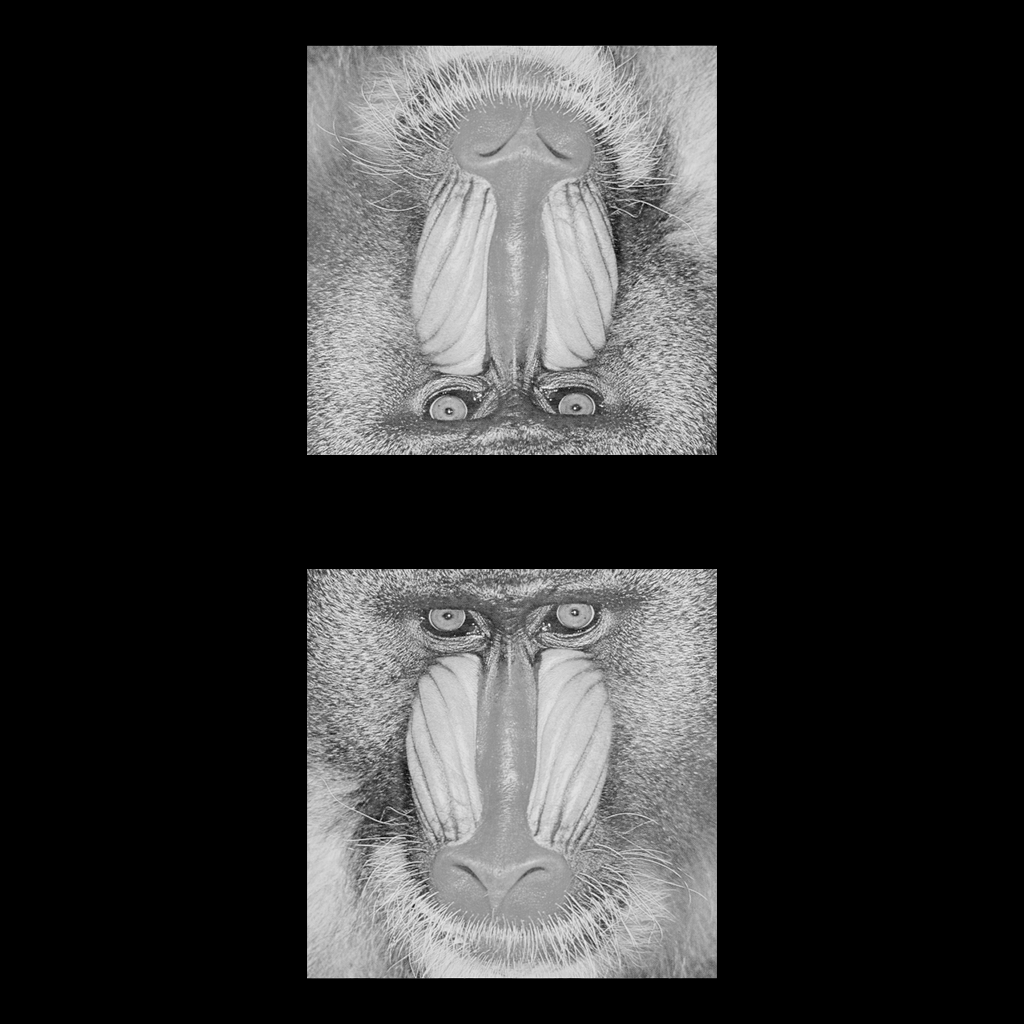
\includegraphics[width=\textwidth]{mandrill_2.png}
    \caption{Target image for the binary-phase SLM}
    \label{fig:mandrill_2}
  \end{subfigure}
  \hfill
  \begin{subfigure}[t]{0.3\textwidth}
    \centering
    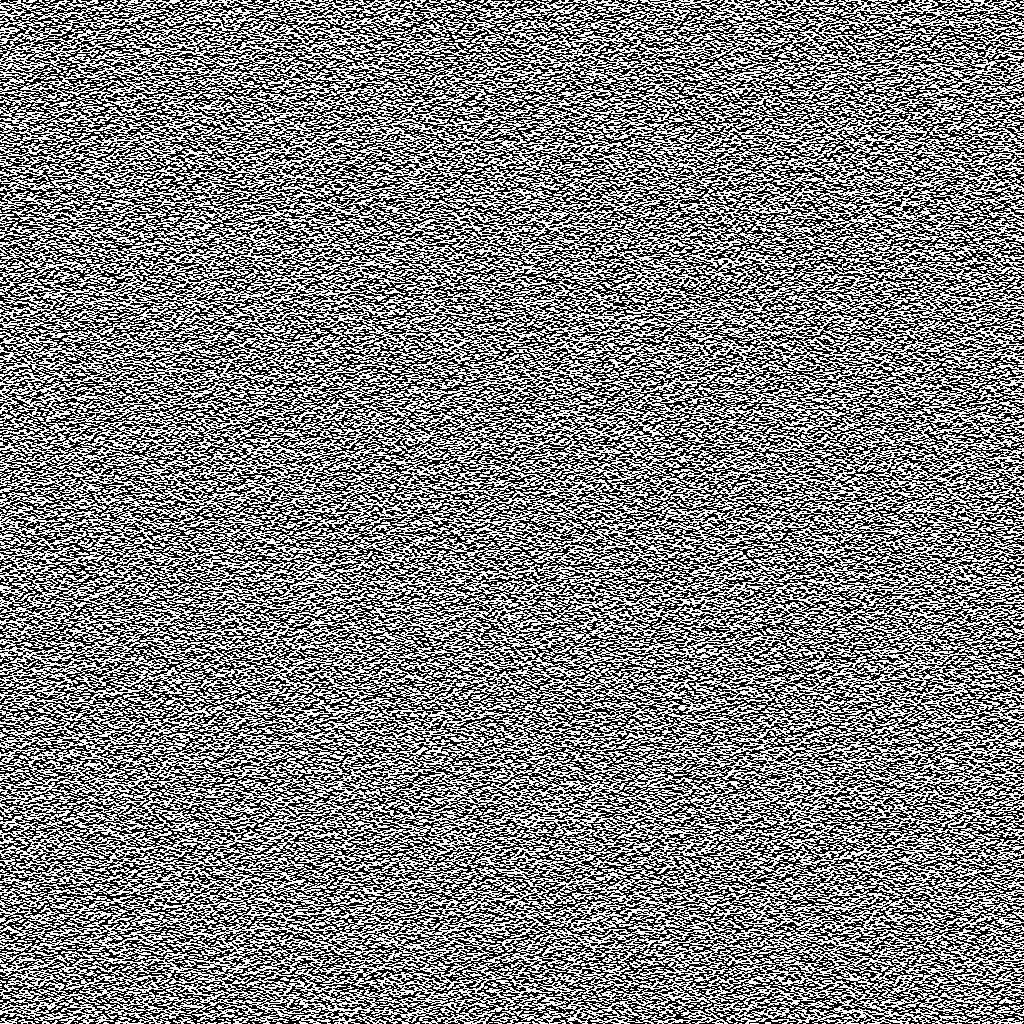
\includegraphics[width=\textwidth]{Naive_binary_Holo.png}
    \caption{Binary-phase Hologram}
    \label{fig:Naive_binary_Holo}
  \end{subfigure}
  \hfill
  \begin{subfigure}[t]{0.3\textwidth}
    \centering
    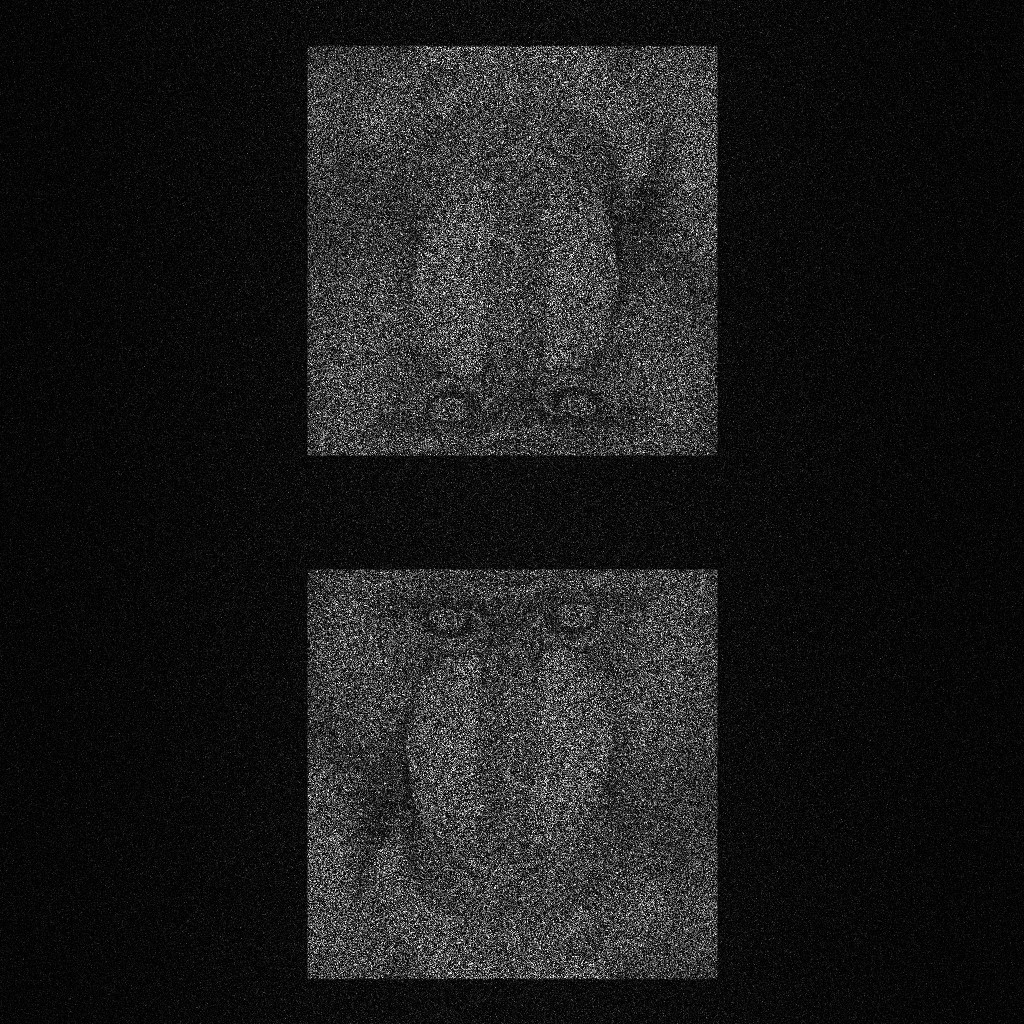
\includegraphics[width=\textwidth]{Naive_binary_Recon.jpg}
    \caption{Reconstruction}
    \label{fig:Naive_binary_Recon}
  \end{subfigure}
  \caption{Output of the improved Phase Unwrapping method with binary-phase quantisation}
  \label{fig:Output of the improved Naive method with binary-phase quantisation}
\end{figure}

The binary phase hologram in \cref{fig:Naive_binary_Holo} is generated by adding an additional binary quantisation step ($\mathcal{Q}$) on the phase hologram computed using \cref{alg:Naive algorithm with random phase}, which is simply rounding all phases to 0 and $\pi$ radians, using \cref{eq:quantisation}
\begin{align}
  \theta_{binary\ quantised}   & \                       \left\{
  \begin{array}{ll}
    0 & -\frac{1}{2} \pi \leqslant \theta < \frac{1}{2} \pi          \\
    \pi & \theta < -\frac{1}{2} \pi \ or\ \theta \geqslant  \frac{1}{2} \pi
  \end{array}
  \right.
  \label{eq:quantisation}
\end{align}
where $\theta$ is the input phase value in range $[-\pi, \pi]$ and $\theta_{binary\ quantised}$ is the output quantised binary phase value. The reconstruction of the binary-phase hologram is shown in \cref{fig:Naive_binary_Recon}, which has an NMSE of \num{4.5452e-07} and an SSIM of 0.0603. To improve the reconstruction quality, better algorithms are needed. The following sections explores predecessors efforts in quality improvement.

\newpage
\subsection{Direct Binary Search (DBS) Algorithm}\label{sec:Direct Binary Search (DBS) Algorithm}
Direct Binary Search (DBS) algorithm \cite{Seldowitz1987} is an algorithm that generates the hologram by randomly flipping each pixel in the SLM between binary states (0 and $\pi$), one by one for many times in order to minimise the difference between its reconstruction intensity $R$ and the target image $T$. The detailed algorithm is described in \cref{alg:DBS algorithm} below:
\begin{algorithm}[H]
  \caption{Direct Binary Search (DBS) algorithm}\label{alg:DBS algorithm}
  \textbf{Input:} Target image $T$, Propagation function $\mathcal{P}$, Loss function $\mathcal{L}$ (e.g. mean-squared error), Number of iterations $N$ \\
  \textbf{Output:} Phase hologram $H$ and its reconstruction intensity $R$
  \begin{algorithmic}
    \State{// Start with a random hologram with a size matching $T$}
    \State $H \gets$ Rand(Size($T$))
    \State $R \gets \vert \mathcal{P}[e^{jH}] \vert ^2$
    \State $L \gets \mathcal{L} [R, T]$

    \For {$n$ = $1$ to $N$}
    \State{// Flip a random pixel in the hologram}
    \State $H_n \gets$ FlipRandomPixel($H$)\\
    \State{// Calculate the loss function for the new hologram}
    \State $R_n \gets \vert \mathcal{P}[e^{jH_n}] \vert ^2$
    \State $L_n \gets \mathcal{L} [R_n, T]$\\
    \State{// Compare the new loss with the old one}
    \If {$L_n < L$}
    \State{// Accept the new hologram if loss is lower}
    \State $H \gets H_n$
    \State $R \gets R_n$
    \State $L \gets L_n$
    \EndIf
    \EndFor
  \end{algorithmic}
\end{algorithm}

Although the DBS algorithm is specifically suited for generating binary phase holograms, it can also be adapted for generating multi-level phase holograms, by representing each level as binary numbers, at the cost of more computation.

\begin{figure}[H]
  \centering
  \begin{subfigure}[t]{0.3\textwidth}
    \centering
    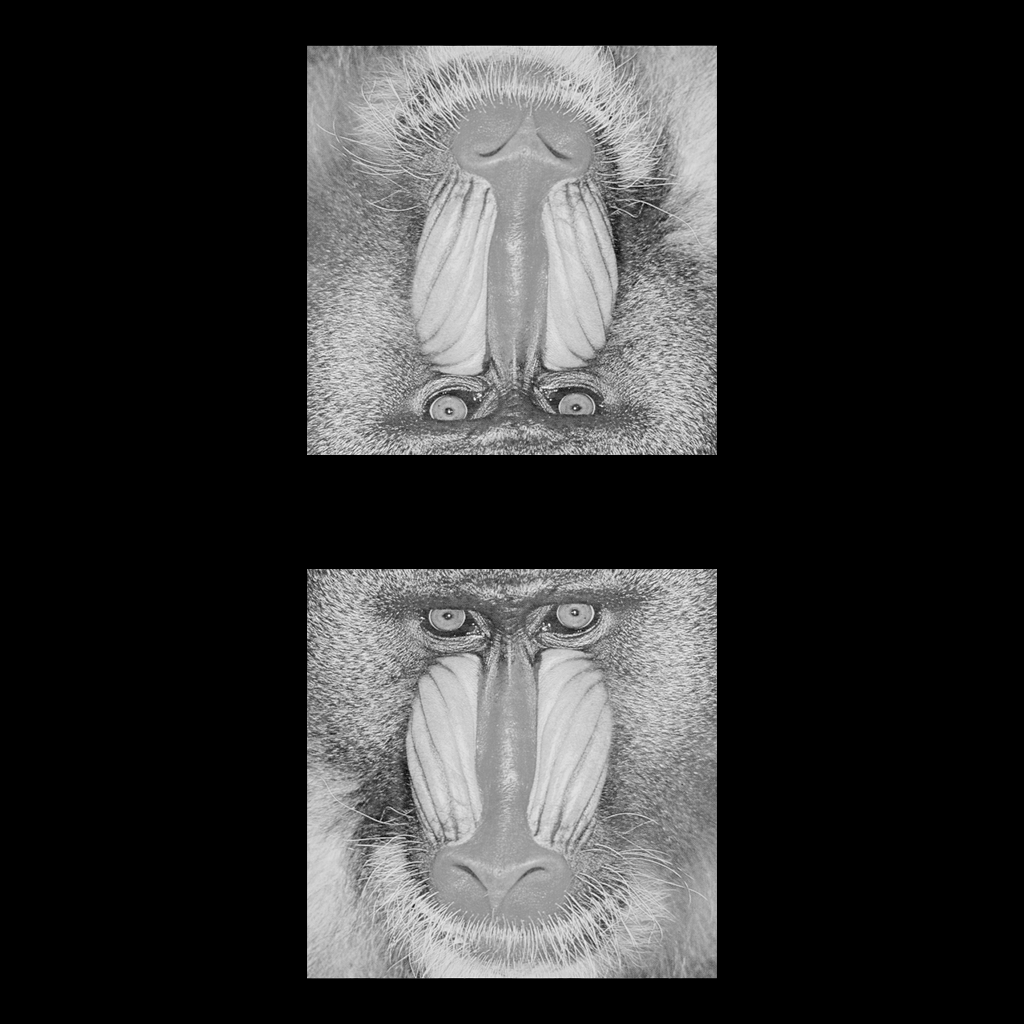
\includegraphics[width=\textwidth]{mandrill_2.png}
    \caption{Target image ($1024 px\times 1024 px$)}
    \label{fig:mandrill_2_DBS}
  \end{subfigure}
  \hfill
  \begin{subfigure}[t]{0.3\textwidth}
    \centering
    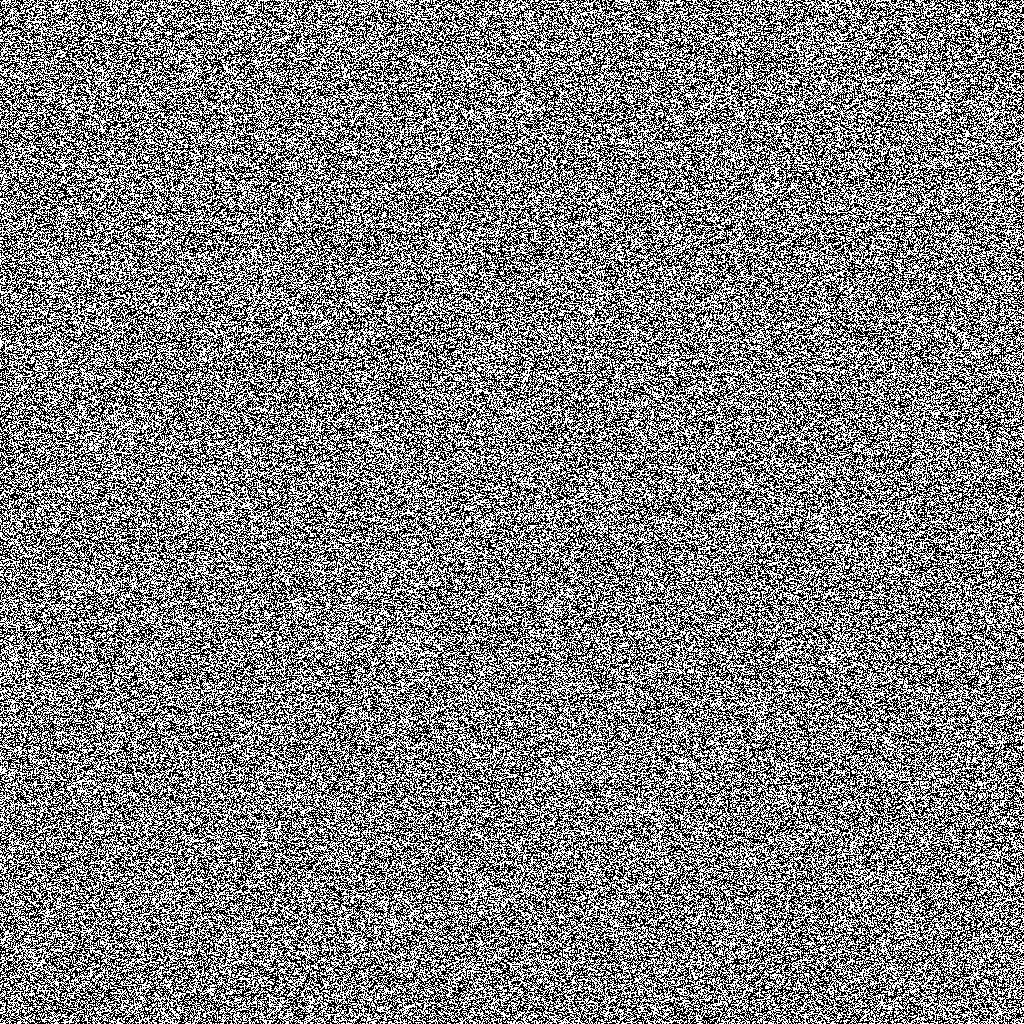
\includegraphics[width=\textwidth]{DBS_mandrill_2_Holo.png}
    \caption{Binary-phase Hologram}
    \label{fig:DBS_mandrill_2_Holo}
  \end{subfigure}
  \hfill
  \begin{subfigure}[t]{0.3\textwidth}
    \centering
    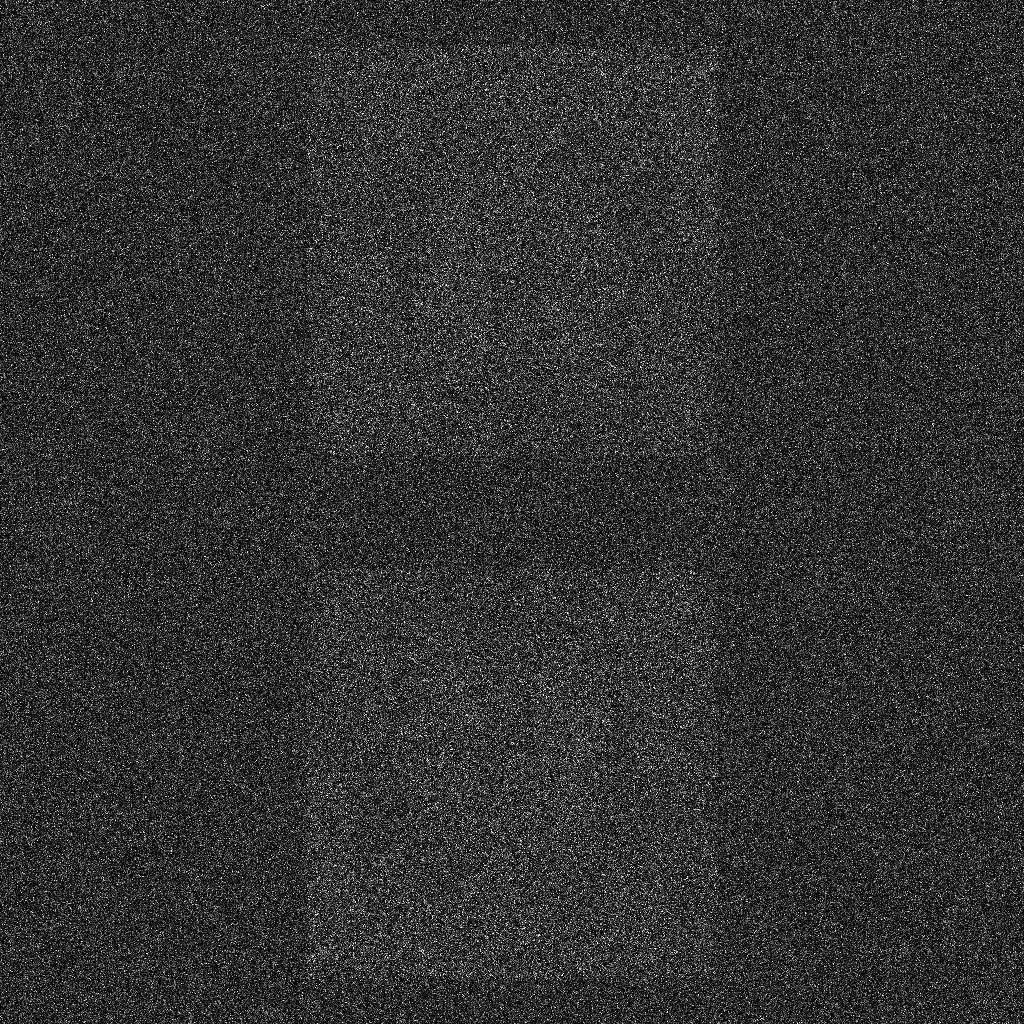
\includegraphics[width=\textwidth]{DBS_mandrill_2_recon_intensity.jpg}
    \caption{Reconstruction}
    \label{fig:DBS_mandrill_2_recon_intensity}
  \end{subfigure}
  \\
  \begin{subfigure}[t]{0.7\textwidth}
    \centering
    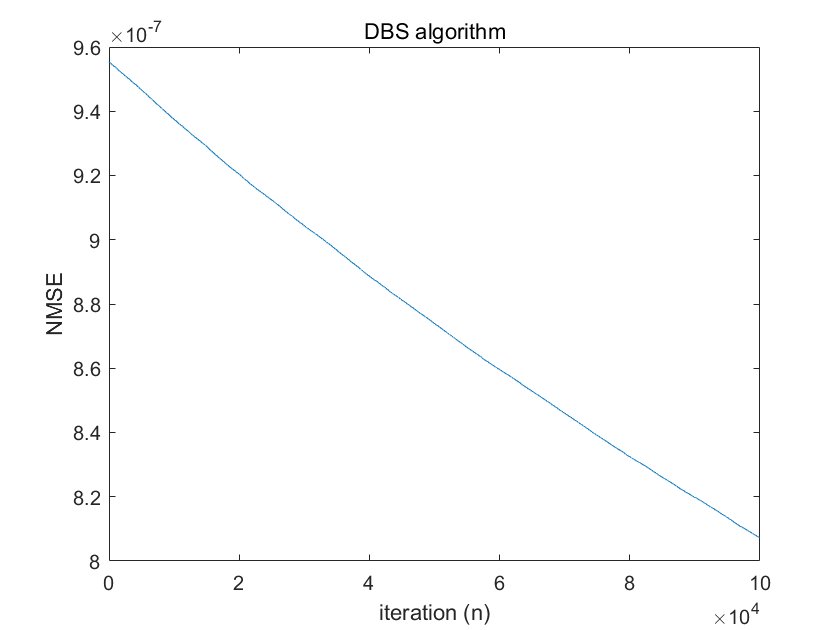
\includegraphics[width=\textwidth]{DBS_mandrill_2_convergence.png}
    \caption{NMSE v.s. iteration plot}
    \label{fig:DBS_mandrill_2_convergence}
  \end{subfigure}
  \caption{DBS algorithm running on the rotationally symmetrical mandrill target}
  \label{fig:DBS algorithm running on the rotationally symmetrical mandrill target}
\end{figure}

DBS algorithm can sometimes find very accurate holograms if the run is lucky; however, it is extremely slow, because it takes numerous iterations (as shown in \cref{fig:DBS_mandrill_2_convergence}, even $10^5$ iterations has not reached a good convergence). The example run on the target image of resolution $1024 px\times 1024 px$ in \cref{fig:mandrill_2_DBS} took more than one hour to finish the $10^5$ iterations, which is still far from convergence. The binary-phase hologram produced is shown in \cref{fig:DBS_mandrill_2_Holo}, and its corresponding reconstruction in \cref{fig:DBS_mandrill_2_recon_intensity} has an NMSE of \num{8.0717e-07} which is 78\% larger than the NMSE of the Phase Unwrapping method being \num{4.5452e-07}. The reconstruction in \cref{fig:DBS_mandrill_2_recon_intensity} has an SSIM of only 0.0076, indicating very poor structural similarity against the target image, and is much worse than the Phase Unwrapping method with SSIM being 0.0603 in \cref{sec:Naive algorithm}.

\begin{figure}[H]
  \centering
  \begin{subfigure}[t]{0.3\textwidth}
    \centering
    
\includegraphics[width=\textwidth]{test_128.png}
    \caption{Target image ($128 px\times 128 px$)}
    \label{fig:test_128}
  \end{subfigure}
  \hfill
  \begin{subfigure}[t]{0.3\textwidth}
    \centering
    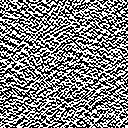
\includegraphics[width=\textwidth]{DBS_test_128_Holo.png}
    \caption{Binary-phase Hologram}
    \label{fig:DBS_test_128_Holo}
  \end{subfigure}
  \hfill
  \begin{subfigure}[t]{0.3\textwidth}
    \centering
    
\includegraphics[width=\textwidth]{DBS_test_128_recon_intensity.png}
    \caption{Reconstruction}
    \label{fig:DBS_test_128_recon_intensity}
  \end{subfigure}
  \\
  \begin{subfigure}[t]{0.7\textwidth}
    \centering
    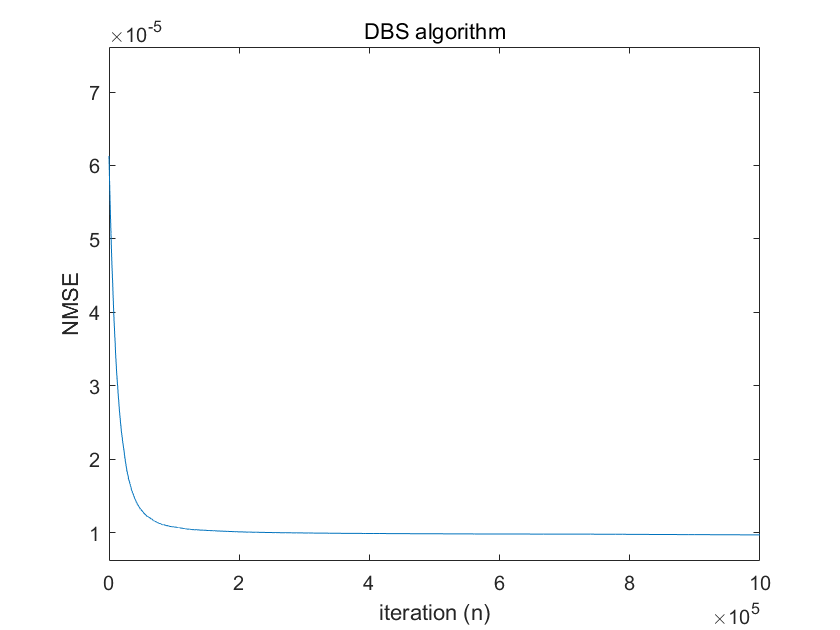
\includegraphics[width=\textwidth]{DBS_test_128_convergence.png}
    \caption{NMSE v.s. iteration plot}
    \label{fig:DBS_test_128_convergence}
  \end{subfigure}
  \caption{DBS algorithm running on the low resolution target}
  \label{fig:DBS algorithm running on the low resolution target}
\end{figure}

As the DBS algorithm only flips one pixel per iteration, it naturally takes significantly longer to generate holograms with higher resolution. To test the programme on a smaller image for much quicker convergence, another target image has been designed as shown in \cref{fig:test_128}, which is also rotationally symmetrical as it is used for the binary-phase hologram generation. After $10^6$ iterations, which took 10 minutes, the hologram generated is shown in \cref{fig:DBS_test_128_Holo} and its resulting reconstruction is shown in \cref{fig:DBS_test_128_recon_intensity}, which has an NMSE of \num{9.6881e-06} and an SSIM of 0.2871. The NMSE v.s. iteration plot in \cref{fig:DBS_test_128_convergence} shows that it reaches a good convergence at around \num{2e5} iterations, corresponding to around 2 minutes. And the curve of NMSE is monotonically decreasing with iteration number, as only holograms with better results are accepted during the iterations.

In summary, the DBS algorithm is a slow but working algorithm for binary phase hologram generation. The programme running time scales up significantly when the target image's resolution gets higher. And also, as it only cares about local optimality at each iteration, it is a greedy algorithm that only follows the steepest descent route, which could easily get trapped in a local minimum where flipping any bit is not getting better reconstruction. Another consequence of the random nature is that the generated hologram will be different at each run, so the quality of the resulting reconstruction ($R$) will depend on how `lucky' each run is. The Simulated Annealing (SA) algorithm \cite{Kirkpatrick1983} in the next session aims to resolve this issue.


\subsection{Simulated Annealing (SA) Algorithm}\label{sec:Simulated Annealing (SA) Algorithm}
The Simulated Annealing (SA) algorithm \cite{Kirkpatrick1983} is a variant of the DBS algorithm. It adopts a probabilistic approach to avoid the steepest gradient descent. Its name derives from the fact that it approximates the recrystallisation process during metal annealing and is particularly well-suited to avoiding the trap of local minima \cite{Yang2009}. To implement this idea, we then need a function ($\mathcal{Z}$) to calculate the probability of the hologram ($H$), and a threshold $p_t$ to decide whether the probability is high enough for the according hologram to be accepted. In this thesis, the probability is selected to be a random function and the threshold is chosen to be 0.9. The pseudocode for this algorithm is listed in \cref{alg:Simulated Annealing (SA) algorithm}.
\begin{algorithm}[H]
  \caption{Simulated Annealing (SA) algorithm}\label{alg:Simulated Annealing (SA) algorithm}
  \textbf{Input:} Target image $T$, Propagation function $\mathcal{P}$, Loss function $\mathcal{L}$, Number of iterations $N$, Probability function $\mathcal{Z}$, Probability threshold $p_t$ \\
  \textbf{Output:} Phase hologram $H$ and its reconstruction intensity $R$
  \begin{algorithmic}
    \State{// Start with a random hologram with a size matching $T$}
    \State $H \gets$ Rand(Size($T$))
    \State $R \gets \vert \mathcal{P}[e^{jH}] \vert ^2$
    \State $L \gets \mathcal{L} [R, T]$

    \For {$n$ = $1$ to $N$}
    \State{// Flip a random pixel in the hologram}
    \State $H_n \gets$ FlipRandomPixel($H$)\\
    \State{// Calculate the loss function for the new hologram}
    \State $R_n \gets \vert \mathcal{P}[e^{jH_n}] \vert ^2$
    \State $L_n \gets \mathcal{L} [R_n, T]$\\
    \State{// Compare the new loss with the old one}
    \If {$L_n < L$}
    \State{// Accept the new hologram if loss is lower}
    \State $H \gets H_n$
    \State $R \gets R_n$
    \State $L \gets L_n$
    \Else
    \State{// Calculate the probability of the hologram}
    \State $p_n \gets \mathcal{Z}[H_n]$
    \If {$p_n > p_t$}
    \State{// Accept the new hologram if the probability exceeds the threshold}
    \State $H \gets H_n$
    \State $R \gets R_n$
    \State $L \gets L_n$
    \EndIf
    \EndIf
    \EndFor
  \end{algorithmic}
\end{algorithm}

\begin{figure}[H]
  \centering
  \begin{subfigure}[t]{0.3\textwidth}
    \centering
    
\includegraphics[width=\textwidth]{test_128.png}
    \caption{Target image ($128 px\times 128 px$)}
    \label{fig:test_128_SA}
  \end{subfigure}
  \hfill
  \begin{subfigure}[t]{0.3\textwidth}
    \centering
    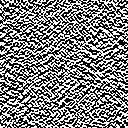
\includegraphics[width=\textwidth]{SA_test_128_Holo.png}
    \caption{Binary-phase Hologram}
    \label{fig:SA_test_128_Holo}
  \end{subfigure}
  \hfill
  \begin{subfigure}[t]{0.3\textwidth}
    \centering
    
\includegraphics[width=\textwidth]{SA_test_128_recon_intensity.png}
    \caption{Reconstruction}
    \label{fig:SA_test_128_recon_intensity}
  \end{subfigure}
  \\
  \begin{subfigure}[t]{0.7\textwidth}
    \centering
    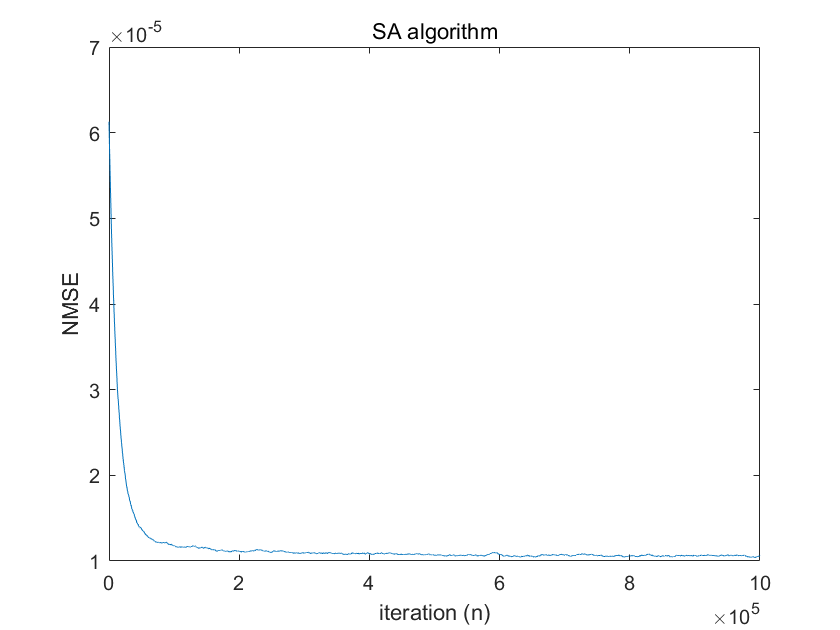
\includegraphics[width=\textwidth]{SA_test_128_convergence.png}
    \caption{NMSE v.s. iteration plot}
    \label{fig:SA_test_128_convergence}
  \end{subfigure}
  \caption{SA algorithm running on the low resolution target}
  \label{fig:SA algorithm running on the low resolution target}
\end{figure}

An implementation of SA algorithm with $p_t = 0.9$ was carried out on the low resolution target in \cref{fig:test_128_SA}, and the resulting binary-phase hologram and its reconstruction are shown in shown in \cref{fig:SA_test_128_Holo} and \cref{fig:SA_test_128_recon_intensity} respectively. From the NMSE v.s. iteration plot in \cref{fig:SA_test_128_convergence}, it can be seen that, instead of the monotonic decrease observed in \cref{fig:DBS_test_128_convergence} for DBS algorithm, the SA algorithm has occasional rises in NMSE, which happens when the probability $p_n$ exceeds the threshold $p_t$. The final NMSE was recorded to be \num{1.0542e-05} and the final SSIM was 0.2750, which are both slightly worse than the DBS algorithm in this case. Due to the probabilistic nature of the SA algorithm, although it can avoid being trapped in local optimal points, the `jump backs' can also cause delays in convergence.

\begin{figure}[H]
  \centering
  \begin{subfigure}[t]{0.3\textwidth}
    \centering
    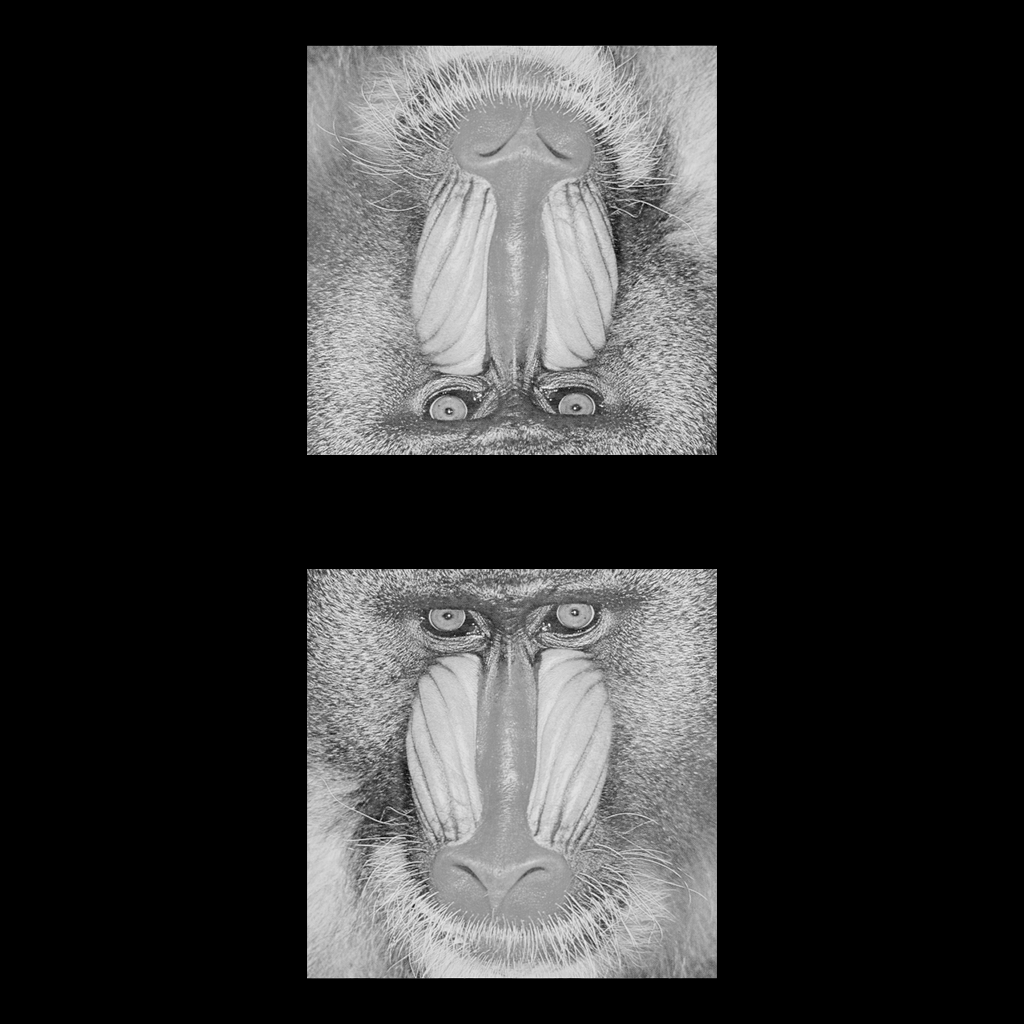
\includegraphics[width=\textwidth]{mandrill_2.png}
    \caption{Target image ($1024 px\times 1024 px$)}
    \label{fig:mandrill_2_SA}
  \end{subfigure}
  \hfill
  \begin{subfigure}[t]{0.3\textwidth}
    \centering
    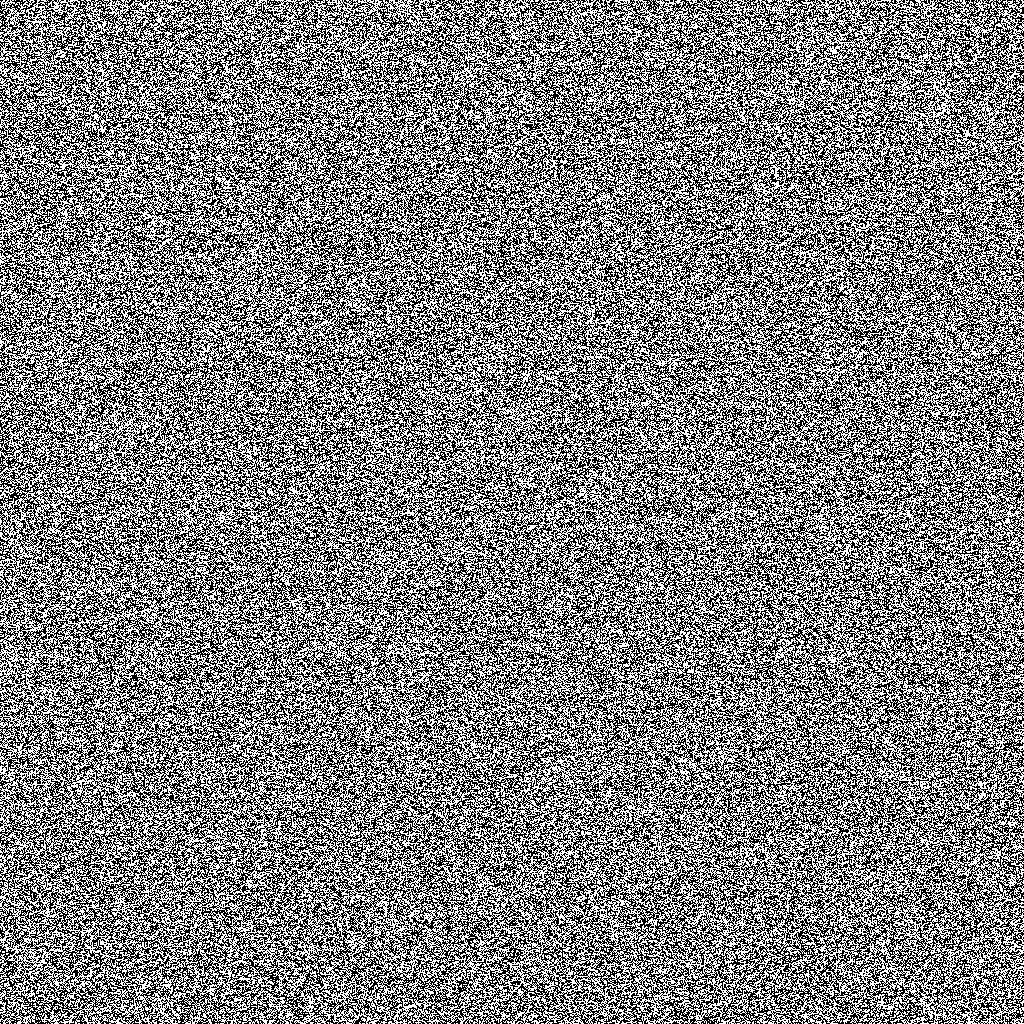
\includegraphics[width=\textwidth]{SA_mandrill_2_Holo.png}
    \caption{Binary-phase Hologram}
    \label{fig:SA_mandrill_2_Holo}
  \end{subfigure}
  \hfill
  \begin{subfigure}[t]{0.3\textwidth}
    \centering
    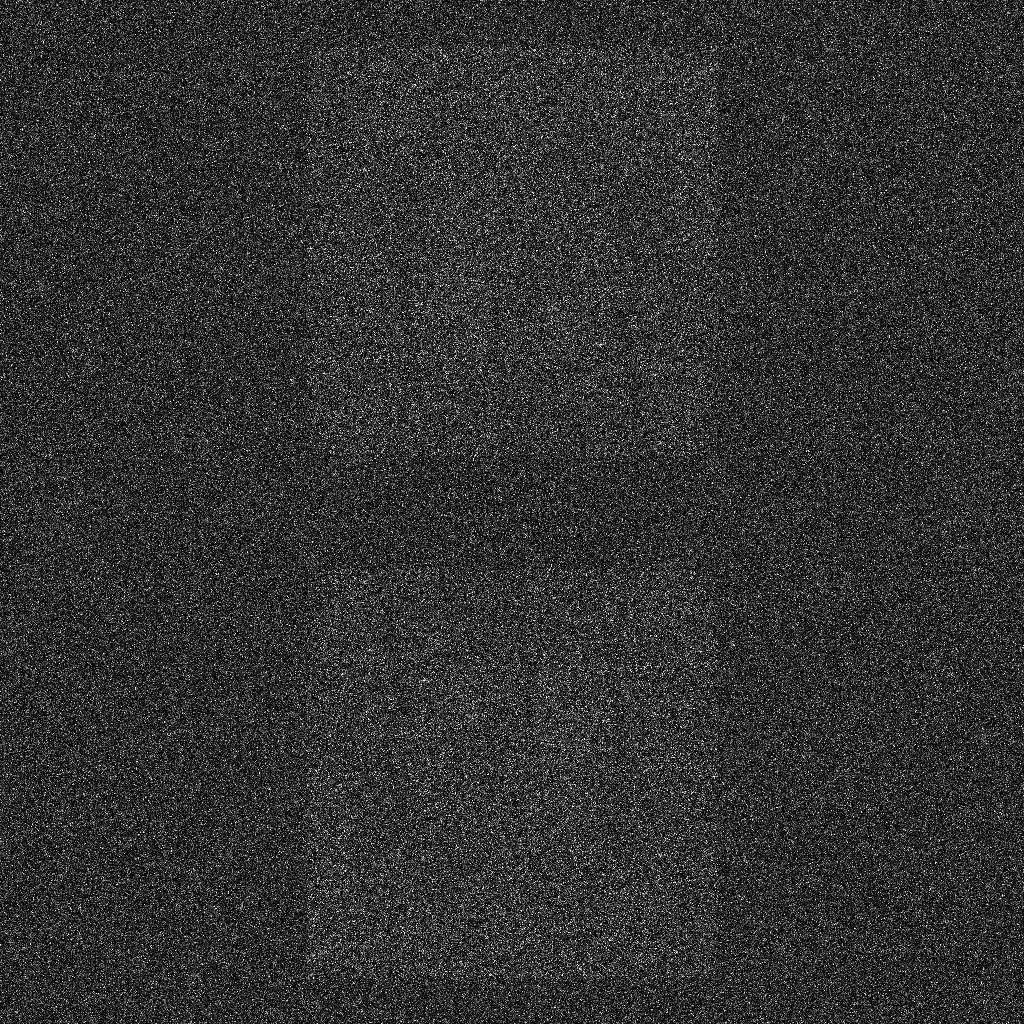
\includegraphics[width=\textwidth]{SA_mandrill_2_recon_intensity.jpg}
    \caption{Reconstruction}
    \label{fig:SA_mandrill_2_recon_intensity}
  \end{subfigure}
  \\
  \begin{subfigure}[t]{0.7\textwidth}
    \centering
    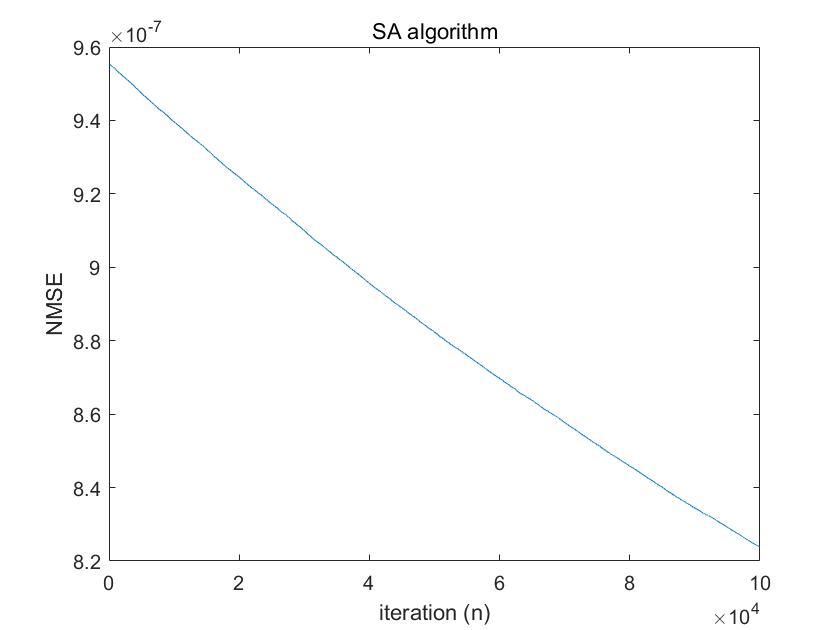
\includegraphics[width=\textwidth]{SA_mandrill_convergence.png}
    \caption{NMSE v.s. iteration plot}
    \label{fig:SA_mandrill_2_convergence}
  \end{subfigure}
  \caption{SA algorithm running on the rotationally symmetrical mandrill target}
  \label{fig:SA algorithm running on the rotationally symmetrical mandrill target}
\end{figure}

Then the SA algorithm was run for the mandrill target in \cref{fig:mandrill_2_SA}. The convergence plot in \cref{fig:SA_mandrill_2_convergence} shows that it did not converge within $10^5$ iterations, which took around one hour. The binary phase hologram generated is shown in \cref{fig:SA_mandrill_2_Holo} and its corresponding reconstruction intensity is shown in \cref{fig:SA_mandrill_2_recon_intensity}, which has an NMSE of \num{8.2054e-07} and an SSIM of 0.0073, which are slightly worse than the DBS algorithm results in \cref{fig:DBS_mandrill_2_recon_intensity} with an NMSE of \num{8.0717e-07} and an SSIM of 0.0076.

Both the DBS and the SA algorithms rely on flipping only a single pixel per iteration, which is very inefficient. A better algorithm should change the values of most pixels at every iteration for better efficiency, and to converge within much fewer iterations for lower computational time. The Gerchberg-Saxton (GS) algorithm \cite{Gerchberg1972} is a classical example, which will be further explained in \cref{sec:Gerchberg-Saxton (GS) Algorithm}.


\subsection{Gerchberg-Saxton (GS) Algorithm}\label{sec:Gerchberg-Saxton (GS) Algorithm}
The Gerchberg-Saxton (GS) algorithm \cite{Gerchberg1972} is a revolutionary algorithm and is much better and more robust than the algorithms introduced in the previous sections. Although being more than 50 years old, the GS algorithm is still frequently used and has lots of variants \cite{Yang1994, WANG2017, Zhou2019}. It functions by iteratively determining the phase profile of the hologram required to reconstruct a target image, looping between the hologram and the reconstruction plane, and applying constraints to each plane accordingly during each iteration. GS algorithm is very easy to implement, its pseudocode is shown in \cref{alg:Gerchberg-Saxton (GS) Algorithm}.

\begin{algorithm}[H]
  \caption{Gerchberg-Saxton (GS) Algorithm}\label{alg:Gerchberg-Saxton (GS) Algorithm}
  \textbf{Input:} Target image $T$, Propagation function $\mathcal{P}$, Number of iterations $N$, Initial phase $\varPhi$ (e.g. random, zeros, or other patterns) \\
  \textbf{Output:} Phase hologram $H$ and its reconstruction intensity $R$
  \begin{algorithmic}
    \State{// Initiate $E$ with amplitude $\sqrt{T}$ and initial phase $\varPhi$}
    \State $E \gets \sqrt{T} \times e^{j\varPhi}$
    \For {$n$ = $1$ to $N$}
    \State{// Compute the hologram plane}
    \State $A \gets \mathcal{P}^{-1}[E]$
    \State{// Apply the phase-only constraint at the hologram plane}
    \State $A \gets e^{j\angle A}$\\
    \State{// Compute the propagation for the new hologram}
    \State $E \gets \mathcal{P}[A]$
    \State{// Apply the target field amplitude constraint at the reconstruction plane}
    \State $E \gets \sqrt{T} \times e^{j\angle E}$
    \EndFor
    \State $H \gets \angle A$
    \State $R \gets \vert \mathcal{P}[A] \vert ^2$
  \end{algorithmic}
\end{algorithm}

\begin{figure}[H]
  \centering
  \begin{subfigure}[t]{0.3\textwidth}
    \centering
    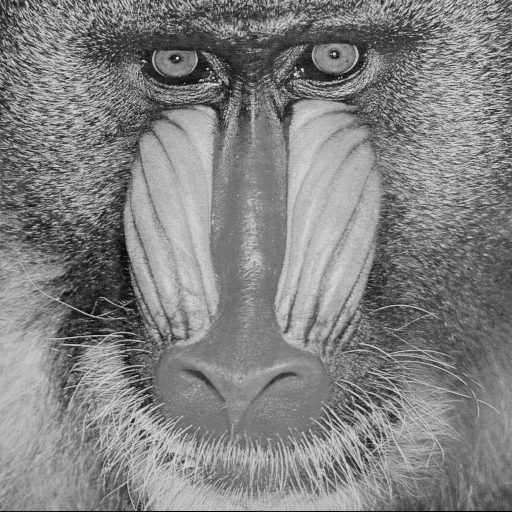
\includegraphics[width=\textwidth]{mandrill.png}
    \caption{Target image ($512 px\times 512 px$)}
  \end{subfigure}
  \hfill
  \begin{subfigure}[t]{0.3\textwidth}
    \centering
    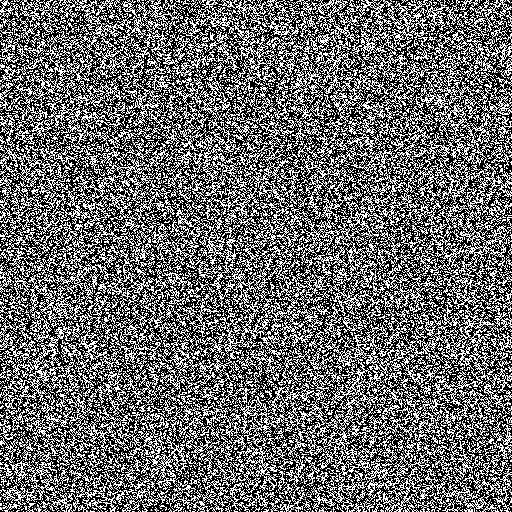
\includegraphics[width=\textwidth]{GS_holo_i_30.png}
    \caption{Multi-level Phase Hologram}
    \label{fig:GS_holo_i_30}
  \end{subfigure}
  \hfill
  \begin{subfigure}[t]{0.3\textwidth}
    \centering
    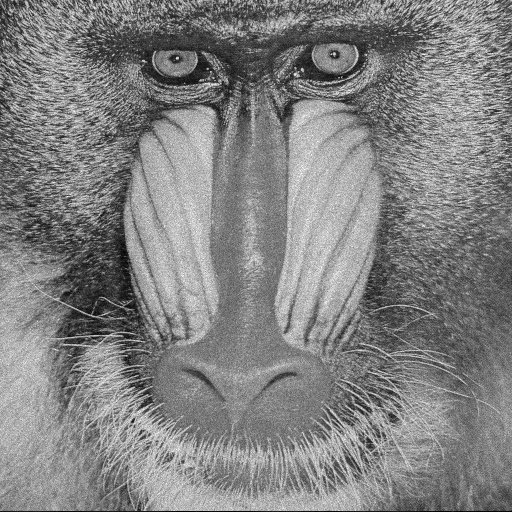
\includegraphics[width=\textwidth]{GS_recon_i_30.png}
    \caption{Reconstruction}
    \label{fig:GS_recon_i_30}
  \end{subfigure}
  \\
  \begin{subfigure}[t]{0.7\textwidth}
    \centering
    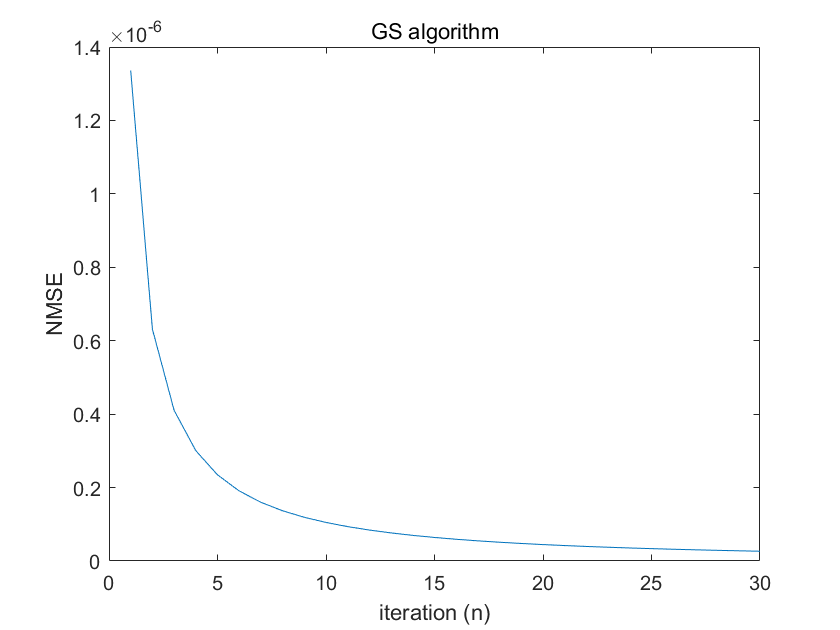
\includegraphics[width=\textwidth]{GS_NMSE_plot.png}
    \caption{NMSE v.s. iteration plot}
    \label{fig:GS_NMSE_plot}
  \end{subfigure}
  \caption{GS algorithm output on the mandrill target}
  \label{fig:GS algorithm output on the mandrill target}
\end{figure}
The GS algorithm described in \cref{alg:Gerchberg-Saxton (GS) Algorithm} was implemented in MATLAB and was first run on the mandrill target image in \cref{fig:mandrill.png}, and the output results are shown in \cref{fig:GS algorithm output on the mandrill target}. \cref{fig:GS_holo_i_30} is the multi-level hologram generated after 30 iterations, and its reconstruction is shown in \cref{fig:GS_recon_i_30}. The reconstruction in \cref{fig:GS_recon_i_30} has an NMSE of \num{2.6612e-08} and an SSIM of 0.7940, which are both much better than the single-iteration Phase Unwrapping method's result in \cref{fig:Naive_rand_recon} (with an NMSE of \num{1.0228e-06} and an SSIM of 0.1603). The NMSE v.s. iteration plot in \cref{fig:GS_NMSE_plot} shows that the GS algorithm converged quickly, providing very good result in tens of iterations, which is much fewer than the DBS and SA algorithms. Although the GS algorithm is more computationally expensive at each iteration, as it needs to compute both a forward and an backward propagation, leading to two Fourier transforms every iteration, the GS algorithm is still much faster and provides much better reconstruction quality than the DBS and SA algorithms.

\begin{figure}[H]
  \centering
  \begin{subfigure}[t]{0.3\textwidth}
    \centering
    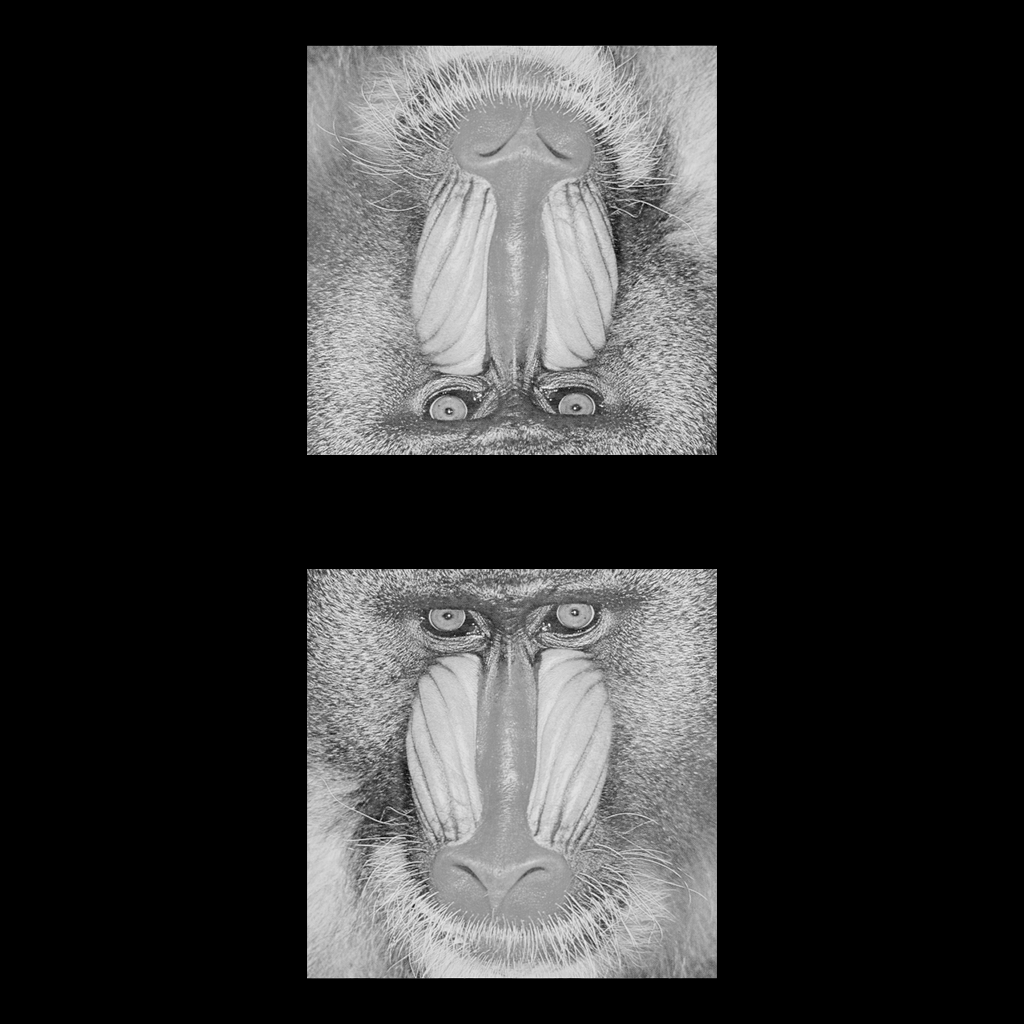
\includegraphics[width=\textwidth]{mandrill_2.png}
    \caption{Target image ($1024 px\times 1024 px$)}
    \label{fig:mandrill_2_GS}
  \end{subfigure}
  \hfill
  \begin{subfigure}[t]{0.3\textwidth}
    \centering
    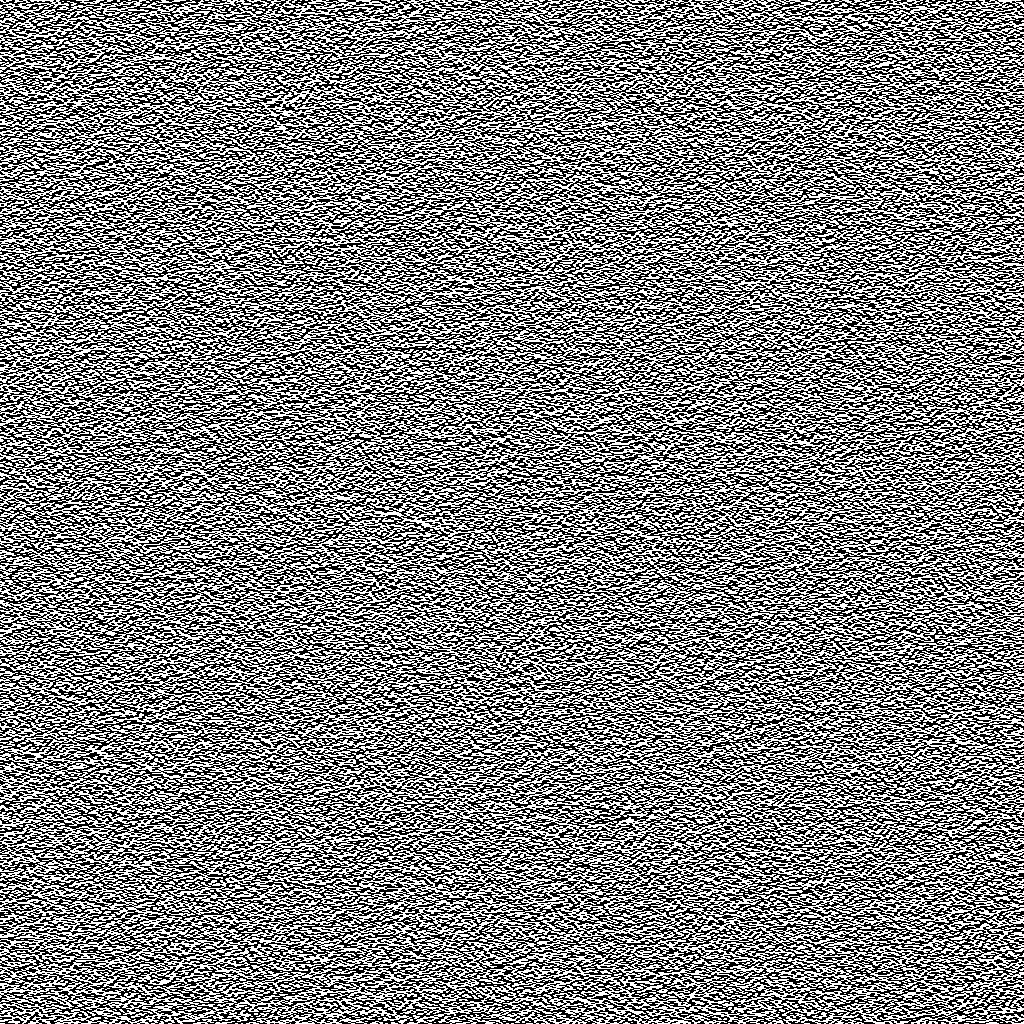
\includegraphics[width=\textwidth]{GS_Holo_mandrill_2.png}
    \caption{Binary-phase Hologram}
    \label{fig:GS_Holo_mandrill_2}
  \end{subfigure}
  \hfill
  \begin{subfigure}[t]{0.3\textwidth}
    \centering
    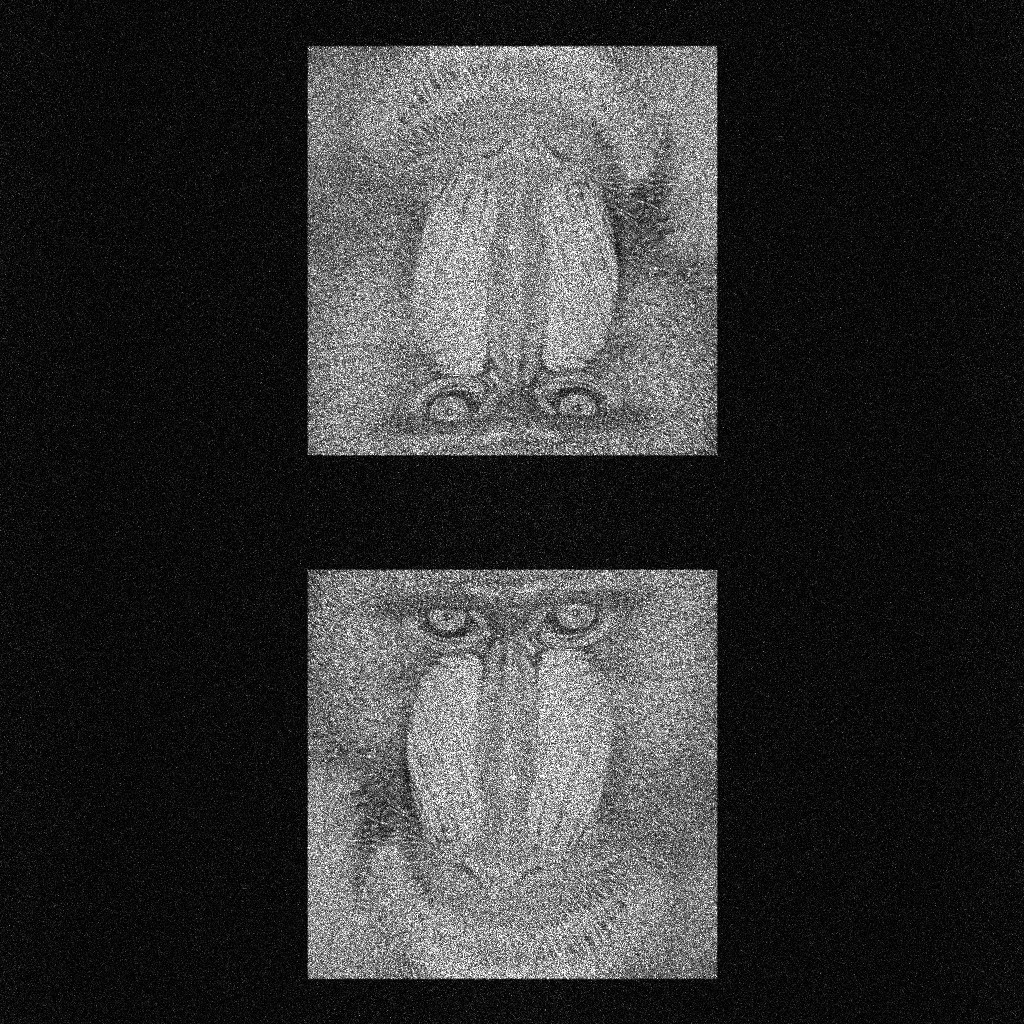
\includegraphics[width=\textwidth]{GS_Recon_mandrill_2.jpg}
    \caption{Reconstruction}
    \label{fig:GS_Recon_mandrill_2}
  \end{subfigure}
  \\
  \begin{subfigure}[t]{0.7\textwidth}
    \centering
    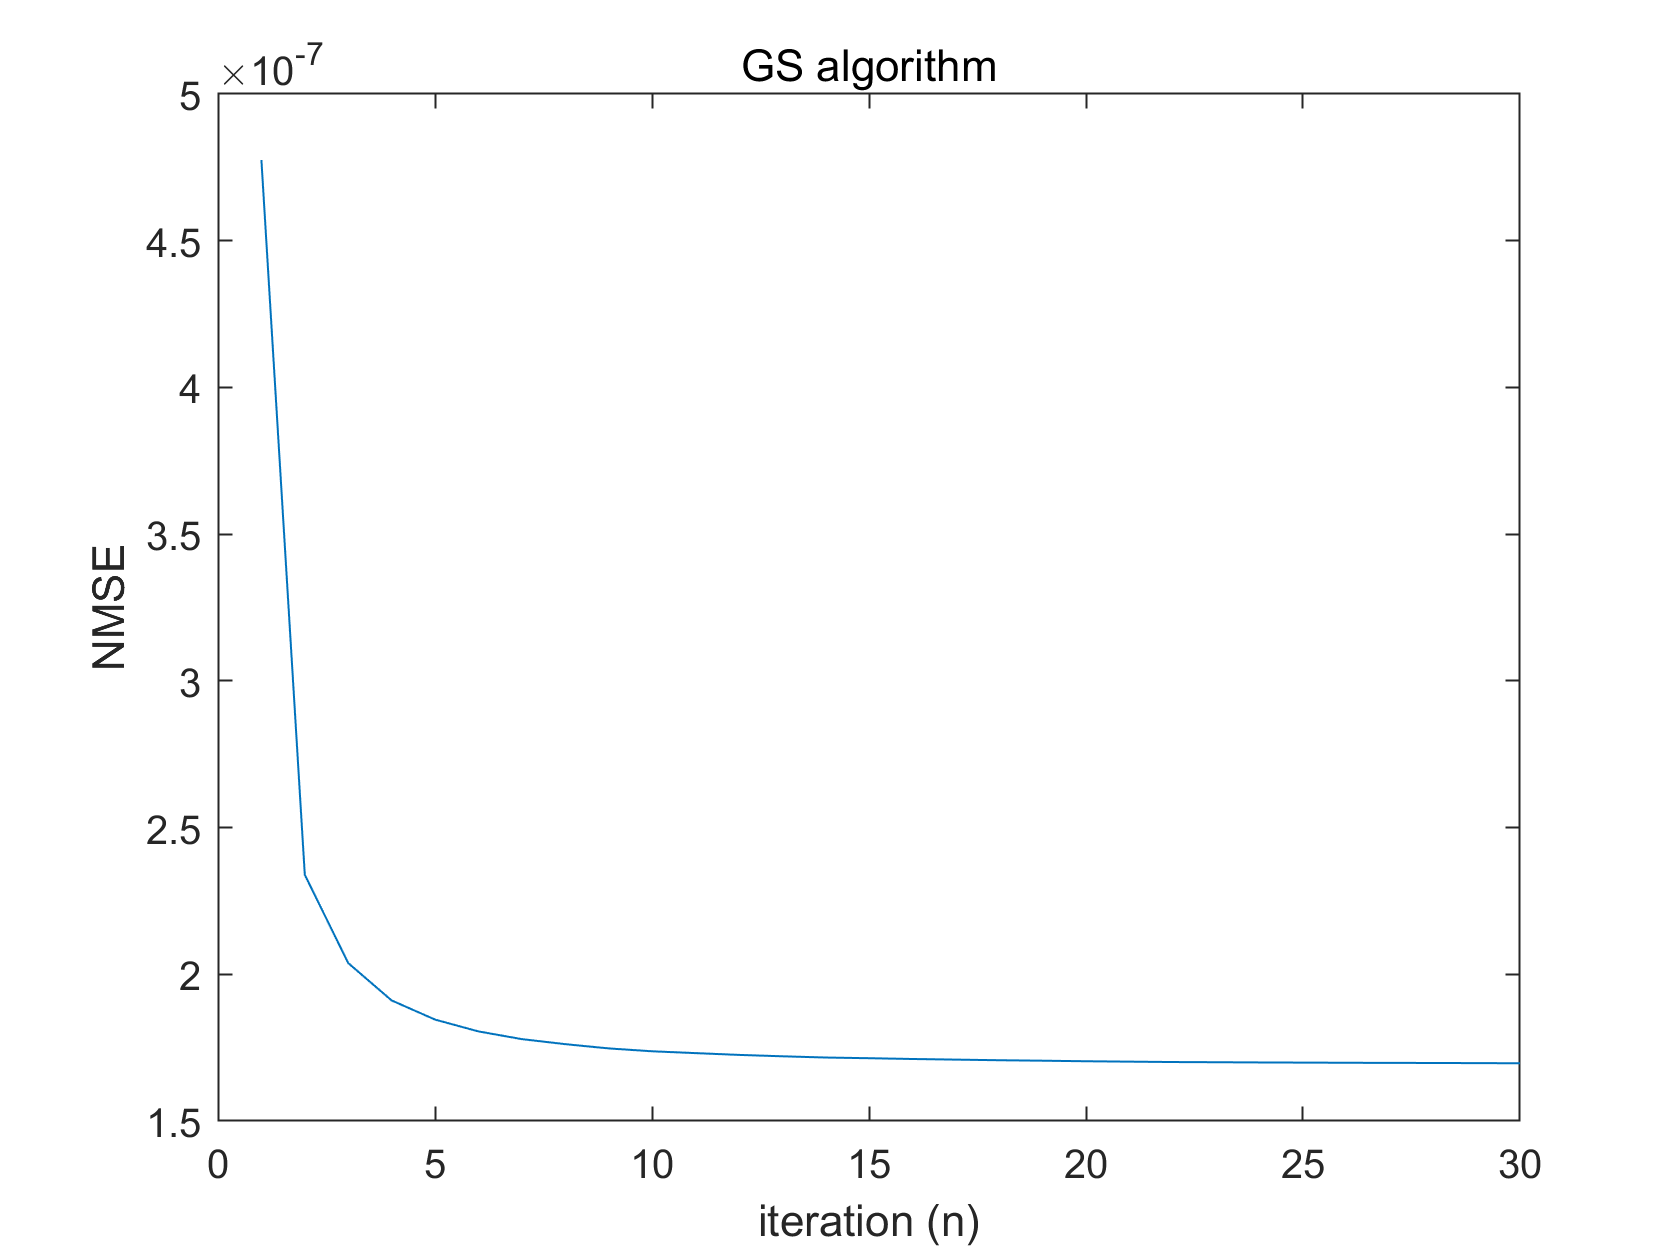
\includegraphics[width=\textwidth]{GS_mandrill_2_convergence.png}
    \caption{NMSE v.s. iteration plot}
    \label{fig:GS_mandrill_2_convergence}
  \end{subfigure}
  \caption{GS algorithm running on the rotationally symmetrical mandrill target}
  \label{fig:GS algorithm running on the rotationally symmetrical mandrill target}
\end{figure}

Then the GS algorithm was adapted to generate binary-phase holograms, for use on the binary-phase SLM in this thesis. The change was simply implemented by adding a quantisation function ($\mathcal{Q}$) when applying the phase-only constraint at the hologram plane (i.e. the line `$A \gets e^{j\angle A}$' in \cref{alg:Gerchberg-Saxton (GS) Algorithm} is changed to `$A \gets e^{j\mathcal{Q}[\angle A]}$'). The results are shown in \cref{fig:GS algorithm running on the rotationally symmetrical mandrill target}. \cref{fig:GS_mandrill_2_convergence} shows good convergence within 20 iterations. The resulting binary-phase hologram is shown in \cref{fig:GS_Holo_mandrill_2} and its corresponding reconstruction in \cref{fig:GS_Recon_mandrill_2} has an NMSE of 1.6968e-07 and an SSIM of 0.0619, which are both better than the Phase Unwrapping method's result in \cref{fig:Output of the improved Naive method with binary-phase quantisation} (with an NMSE of \num{4.5452e-07} and an SSIM of 0.0603). In summary, the GS algorithm is quick and robust. On my laptop computer of model ASUS ROG Zephyrus M16, which has a CPU of model i7-11800H and a GPU of model RTX3060, the 30 iterations took 1.5 seconds to complete. It reached convergence in tens of iterations. However, as it is still iterative, generating holograms in real-time is still a challenge, and the reconstruction still suffers from noise.


\subsection{One-Step Phase Retrieval (OSPR) Algorithm}\label{sec:One Step Phase Retrieval (OSPR) Algorithm}
The OSPR algorithm was first demonstrated by Cable and Buckley \cite{Cable2004}. It is a solution to high-quality hologram reconstruction that relies on time multiplexing of holograms, exploiting the response time of eye in order to reduce noise in the replay field \cite{Cable2006}. The random noise is averaged by the eye, while the target image stays, so that the average noise can be reduced. The perceived noise is lessened by the temporal average detected by the eye, rather than computational optimisation of the hologram \cite{Cable2006}. The pseudocode for OSPR is shown in \cref{alg:One-Step Phase Retrieval (OSPR) algorithm} below.

\begin{algorithm}[H]
  \caption{One-Step Phase Retrieval (OSPR) algorithm}\label{alg:One-Step Phase Retrieval (OSPR) algorithm}
  \textbf{Input:} Target image $T$, Propagation function $\mathcal{P}$, Number of sub-frames $S$, Quantisation function $\mathcal{Q}$\\
  \textbf{Output:} List of phase holograms $H[1\ldots S]$
  \begin{algorithmic}
    \State // Compute a list of hologram sub-frames
    \For {$i$ = $1$ to $S$}
    \State $E \gets \sqrt{T} \cdot $ RandomPhase()
    \State $A \gets \mathcal{P}^{-1}[E]$
    \State $H[i] \gets \mathcal{Q}[\angle A]$
    \EndFor\\
    \State // Then display the sub-frames on the phase modulator sequentially
    \State $i\gets 1$
    \While {True}
    \State Display($H[i]$)
    \State $i\gets i + 1$
    \If {$i > S$}
    \State $i\gets 1$
    \EndIf
    \EndWhile
  \end{algorithmic}
\end{algorithm}

When generating the list of holograms, it repetitively computes the inverse propagation of the target amplitude (which is the square-root of the target intensity $T$) multiplied by different random phases, for a total of $S$ times to generate $S$ hologram sub-frames ($H[1\ldots S]$). The computation of each hologram sub-frame is the same as the Phase Unwrapping method in \cref{alg:Naive algorithm with random phase} discussed in \cref{sec:Naive algorithm}. Then the $S$ hologram sub-frames are displayed sequentially on a SLM having a refresh rate being so fast that the average reconstruction intensity is perceived by the human eyes. As currently available fast SLMs are binary-phase modulators, an example run on the rotationally symmetrical target previously used in \cref{fig:mandrill_2_DBS} was carried out for 24 sub-frames ($S=24$). The results are summarised in \cref{fig:ospr_mandrill_2}.

\begin{figure}[H]
	\centering
	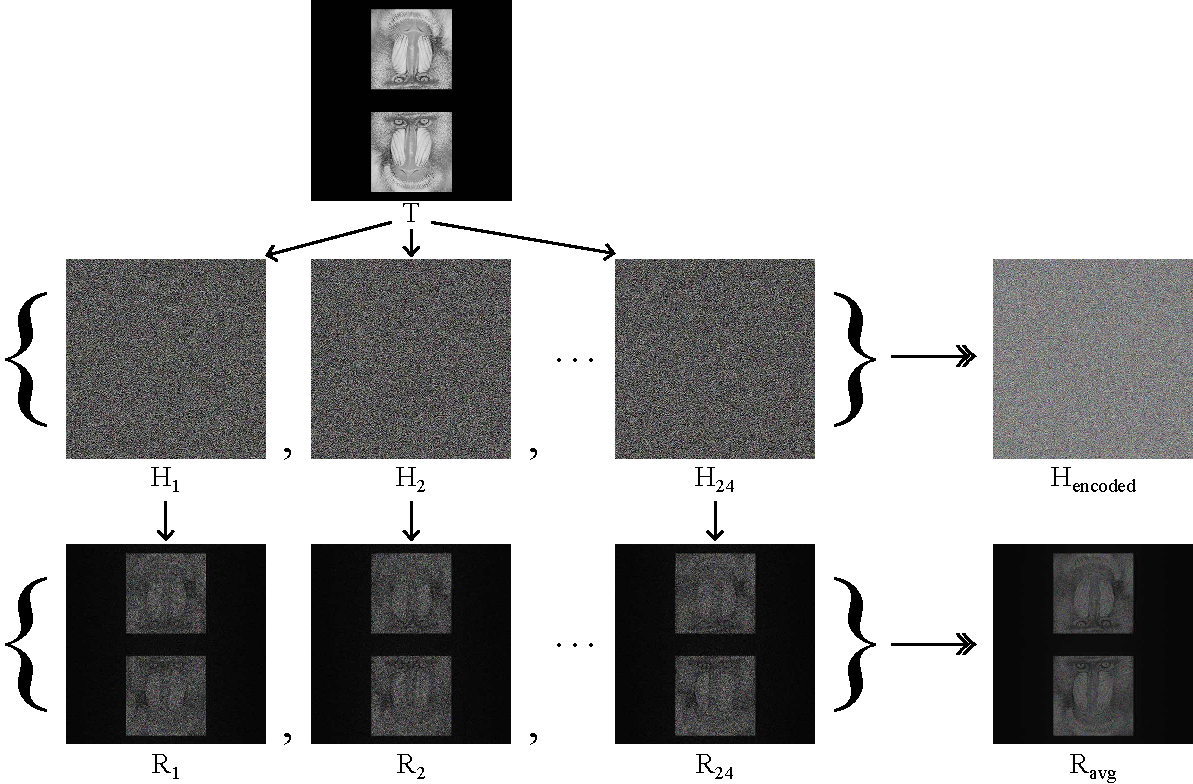
\includegraphics[width=1.0\textwidth]{ospr_mandrill_2.pdf}
	\caption{OSPR algorithm running on the rotationally symmetrical mandrill target}
	\label{fig:ospr_mandrill_2}
\end{figure}

In \cref{fig:ospr_mandrill_2}, a total of 24 binary-phase hologram sub-frames ($H_1, H_2, \ldots, H_{24}$) were generated for the target image $T$. For easier data transfer and to fit with the common display signal formats, the 24 binary-phase hologram sub-frames are encoded into a single file with 8 bit depth and RGB (red-green-blue) channels, so that each of the $(8\times 3 = )24$ bit-planes corresponds to a single binary-phase hologram sub-frame. For a quantitative analysis, the reconstruction intensities of the hologram sub-frames are computed in $R_1, R_2, \ldots, R_{24}$ respectively, whose average is $R_{avg}$ in \cref{fig:ospr_mandrill_2}. The average reconstruction intensity $R_{avg}$ has an NMSE of \num{9.8632e-08} and an SSIM of 0.1321, which are both significantly better than the GS algorithm (NMSE=\num{1.6968e-7}, SSIM=0.0619) and the Phase Unwrapping method (NMSE=\num{4.5452e-7}, SSIM=0.0603).

The major advantage of the OSPR algorithm is that it is fast. It is non-iterative and requires only one Fourier Transform per frame, taking less than a second to generate a 24-frame hologram set. Its non-iterative nature also allows it to be parallelised to further improve computation speed, which is crucial for Light Blue Optics who made a real-time holographic laser projector commercially available in 2010 \cite{Buckley2008}, although the product was later discontinued for financial reasons. The downside of this algorithm is that the sub-frames are independent from each other, and the final reconstruction output is still subject to some noise, as they are only more randomly distributed instead of being reduced. There is a variant of improvement on the OSPR algorithm, called Adaptive OSPR (AD-OSPR), to be introduced in \cref{sec:Adaptive One-Step Phase Retrieval (AD-OSPR) Algorithm}.



\subsection{Adaptive One-Step Phase Retrieval (AD-OSPR) Algorithm}\label{sec:Adaptive One-Step Phase Retrieval (AD-OSPR) Algorithm}

The AD-OSPR algorithm \cite{Kaczorowski2016} is a variant of the OSPR algorithm. It aims to improve the reconstruction quality without introducing a significant amount of additional computational cost. It functions in such a way that, when computing the second sub-frame onwards, it subtracts the average reconstruction from the target image to get the error, so that it can compensated in the next iteration. To help explain the process in detail, a pseudocode is written for the AD-OSPR algorithm, as shown in \cref{alg:Adaptive One-Step Phase Retrieval (AD-OSPR) algorithm}.

\begin{algorithm}[H]
  \caption{Adaptive One-Step Phase Retrieval (AD-OSPR) algorithm}\label{alg:Adaptive One-Step Phase Retrieval (AD-OSPR) algorithm}
  \textbf{Input:} Target image $T$, Propagation function $\mathcal{P}$, Number of sub-frames $S$, Quantisation function $\mathcal{Q}$\\
  \textbf{Output:} List of phase holograms $H[1\ldots S]$
  \begin{algorithmic}
    \State // Compute a list of hologram sub-frames
    \State $T[1] \gets T$
    \State $R_{total} \gets 0$
    \For {$i$ = $1$ to $S$}
    \State $E \gets \sqrt{T[i]} \cdot$ RandomPhase()
    \State $A \gets \mathcal{P}^{-1}[E]$
    \State $H[i] \gets \mathcal{Q}[\angle A]$
    \State // Compute the reconstruction intensity
    \State $R \gets \vert \mathcal{P}[e^{jH[i]}] \vert ^2$
    \State // Carry out energy conservation to match the total energy of the target image
    \State $R \gets R \cdot \sqrt{\frac{sum(T^2)}{sum(R^2)}} $ // squares and sums are taken element wise
    \State // Compute the total reconstruction intensity so far
    \State $R_{total} \gets R_{total} + R$
    \State // Compute the new target for the next iteration
    \For {$[x, y]$ = $[1, 1]$ to size($T$)} // loop among all the pixels
    \If {($i+1)\cdot T[x,y]$ > $R_{total}[x,y]$}
    \State $T[i+1][x,y] \gets (i+1)\cdot T[x,y] - R_{total}[x,y]$
    \Else
    \State $T[i+1][x,y] \gets 0$
    \EndIf
    \EndFor

    \EndFor
    \State // Then display the sub-frames on the phase modulator sequentially
    \State $i\gets 1$
    \While {True}
    \State Display($H[i]$)
    \State $i\gets i + 1$
    \If {$i > S$}
    \State $i\gets 1$
    \EndIf
    \EndWhile
  \end{algorithmic}
\end{algorithm}

In the pseudocode in \cref{alg:Adaptive One-Step Phase Retrieval (AD-OSPR) algorithm}, the target intensity for the first iteration ($T[1]$) is initialised as the input target image $T$, and the total reconstruction intensity for the holograms generated up to each iteration ($R_{total}$) is initialised as 0. Then the $\textbf{for}$ loop starts from the same routine as the OSPR algorithm, multiplying a random phase to the square root of target intensity, taking an inverse propagation, and applying the binary phase quantisation. Then, the total reconstruction is computed by forward propagating the quantised hologram, conserving the energy to match the target image, and adding to the total reconstruction of the last iteration. The total reconstruction is then used to compute the target intensity for the next iteration, by subtracting the total reconstruction from $(i+1)$ times the target image, with an $\textbf{if-else}$ statement to avoid negative intensity values. To provide a visual illustration, an example run of the AD-OSPR algorithm was carried out on the mandrill target as shown in \cref{fig:adospr_mandrill_2}.

\begin{figure}[H]
	\centering
	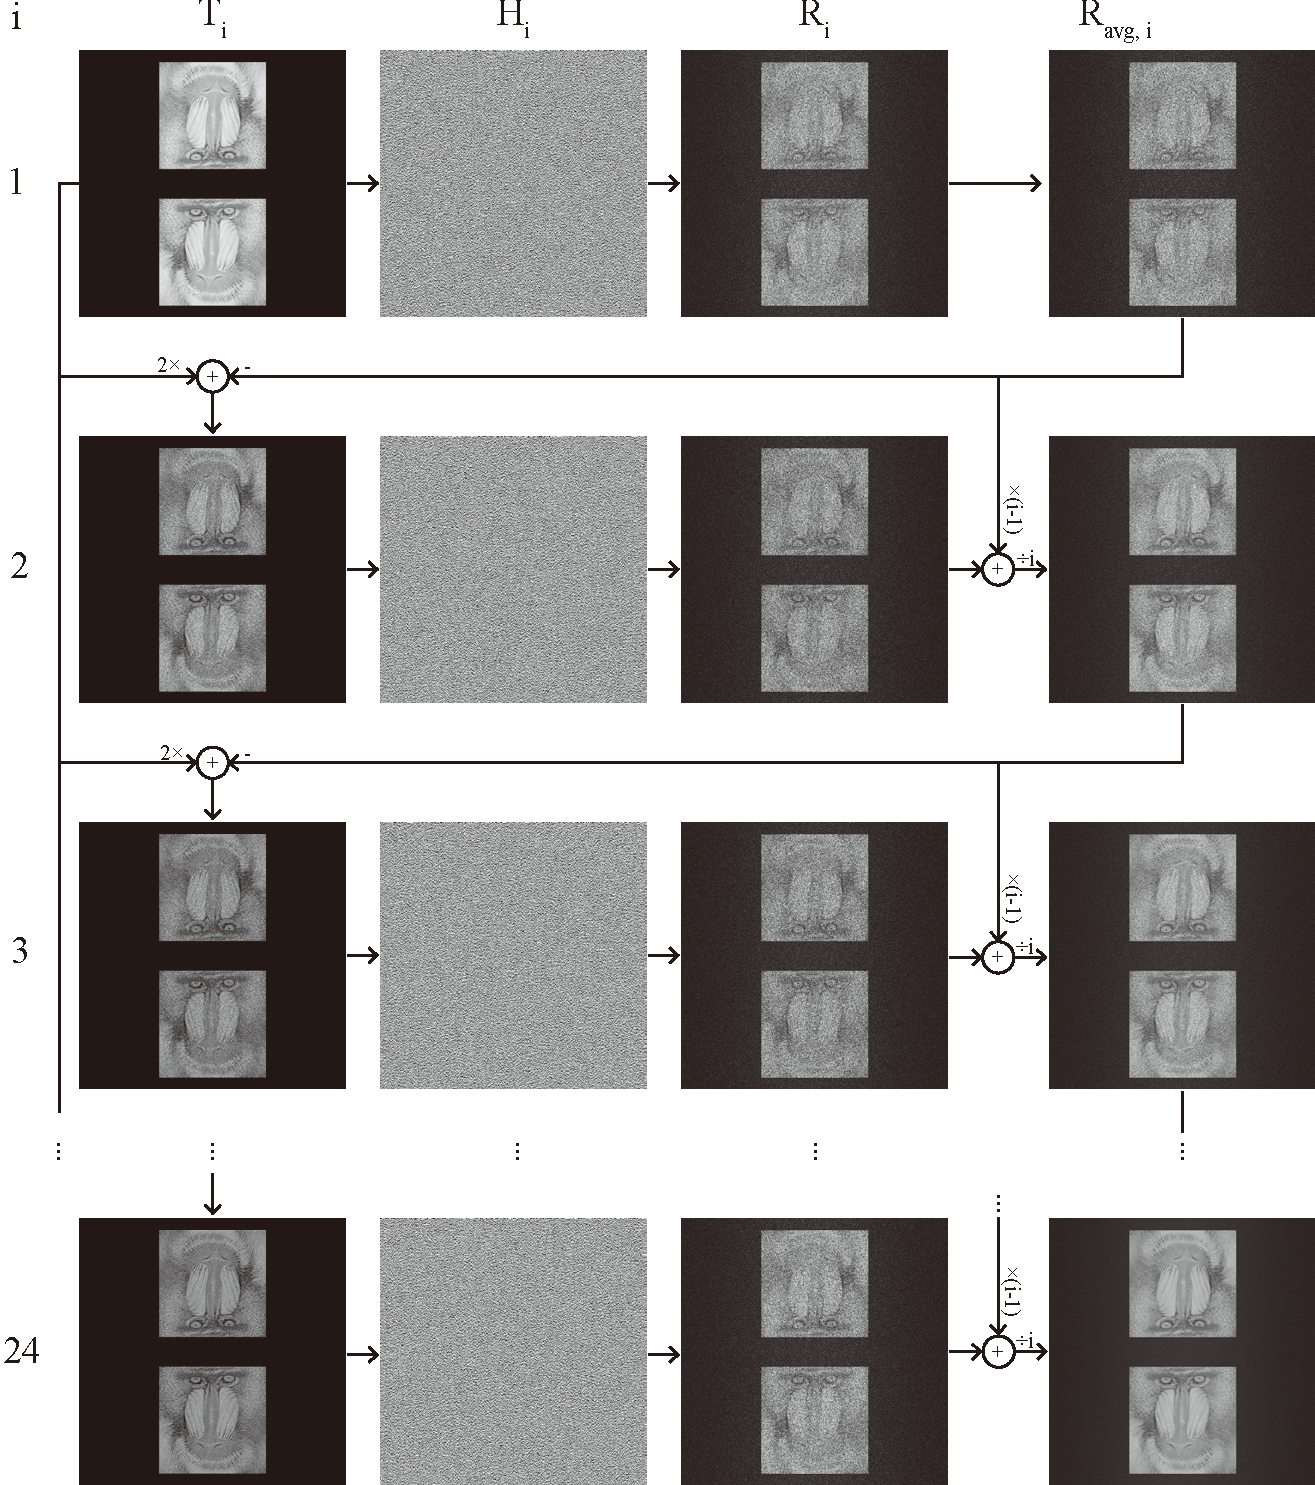
\includegraphics[width=1.0\textwidth]{adospr_mandrill_2.pdf}
	\caption{AD-OSPR algorithm running on the rotationally symmetrical mandrill target}
	\label{fig:adospr_mandrill_2}
\end{figure}

In \cref{fig:adospr_mandrill_2}, each row of images correspond to one iteration that is indexed in the `i' column, where only iterations 1, 2, 3, 24 are shown here, while iterations 4-23 are omitted to save space. At each iteration, the binary-phase hologram $H_i$ is computed from its target $T_i$, and the corresponding reconstruction is shown in $R_i$. Instead of showing the $R_{total, i}$, the $R_{avg, i}=\frac{R_{total, i}}{i}$ is shown here as $R_{total, i}$ has increasing dynamic range at each iteration.

For the first iteration, the target image of the same one as in \cref{fig:ospr_mandrill_2} is used, and the first average reconstruction $R_{avg, 1}$ is just the first reconstruction $R_1$. Then, from the second iteration onwards, the target intensity $T_i$ is updated following the pseudocode in \cref{alg:Adaptive One-Step Phase Retrieval (AD-OSPR) algorithm}. After 24 iterations, the 24 hologram sub-frames are computed and their average reconstruction ($R_{avg, 24}$) had an NMSE of \num{9.1161e-08} and a SSIM of 0.1992, which are both better than the OSPR algorithm in \cref{sec:One Step Phase Retrieval (OSPR) Algorithm} who achieved an NMSE of \num{9.8632e-08} and an SSIM of 0.1321.

The programme running time of the AD-OSPR algorithm is nearly the same as the OSPR algorithm, both being around 0.7 second. Therefore the AD-OSPR algorithm is quite an effective improvement on the original OSPR algorithm, achieving a 7.6\% reduction in NMSE and 50.8\% improvement in SSIM without adding much computation. The disadvantage is however, that it cannot be parallelised, unlike the OSPR algorithm, as it needs to have the total reconstruction intensity result from the previous iteration for use in the next iteration.


\newpage
\subsection{3D CGH}
\cref{sec:Naive algorithm} - \cref{sec:Adaptive One-Step Phase Retrieval (AD-OSPR) Algorithm} described several algorithms to generate a phase hologram for a single target image. However, the major benefit of holography is that it can produce a true 3D light field, much more than just a single slice 2D image. Then the problem arises as how to generate a hologram for 3D targets to make full use of the major benefit of holography. The simplest method is to slice the 3D target into a set of 2D layers, like computed tomography (CT) scanning, and then generate a hologram so that its Fresnel propagation (in \cref{eq:fresnel-diffraction}) at each depth ($z$) matches the according layer. This subsection therefore reviews how the current methods in \cref{sec:Naive algorithm} - \cref{sec:Adaptive One-Step Phase Retrieval (AD-OSPR) Algorithm} can be adapted to multi-depth hologram generation.

\begin{figure}[H]
	\centering
	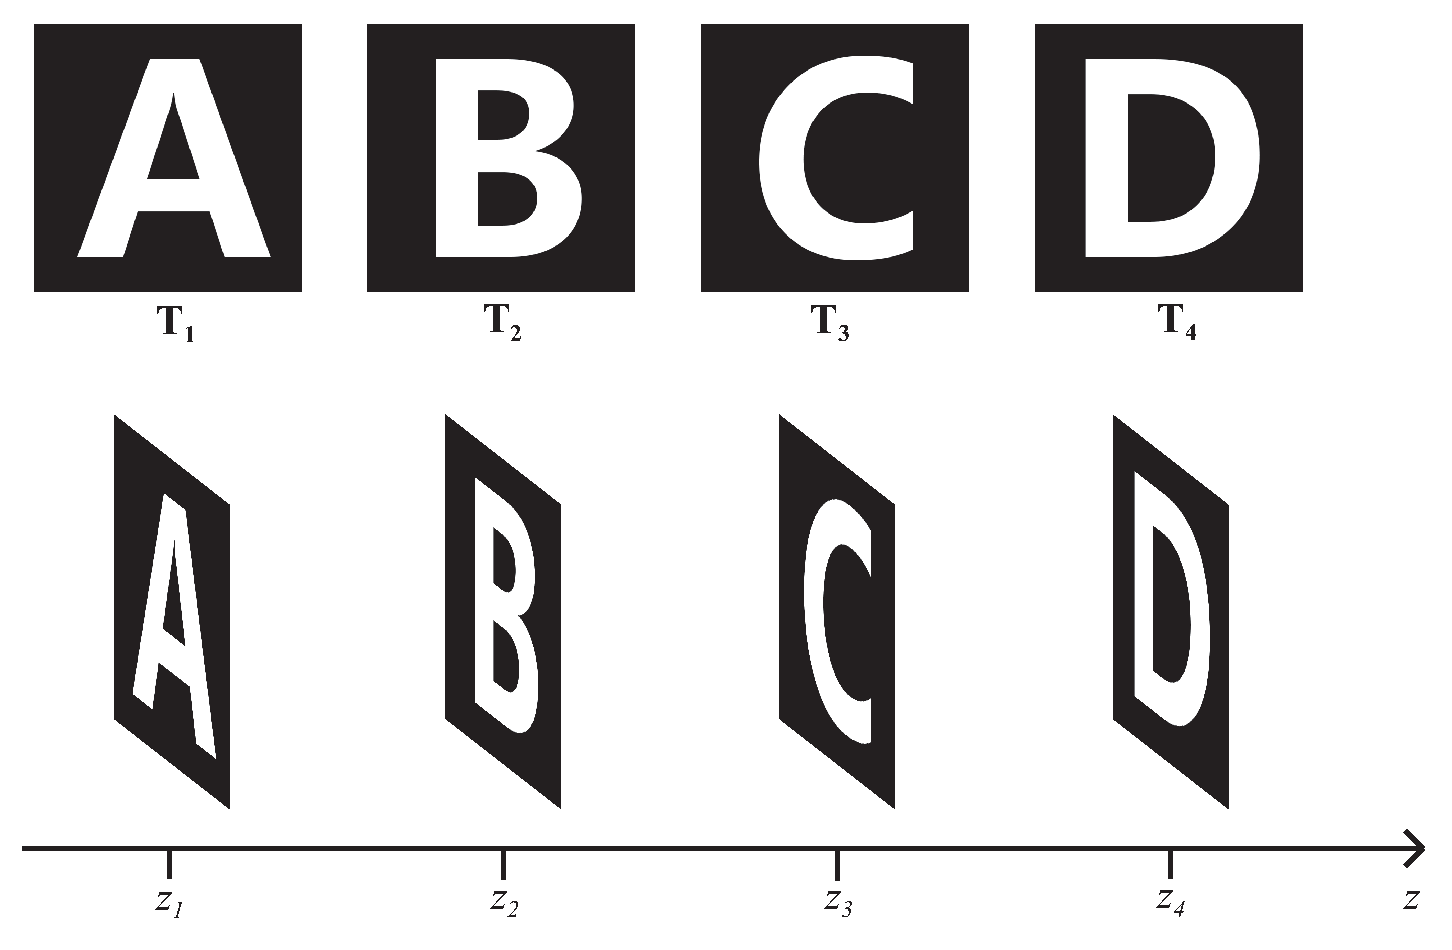
\includegraphics[width=1.0\textwidth]{ABCD/ABCD_target.eps}
	\caption{Multi-slice target consisted of 4 different characters at different distances}
	\label{fig:ABCD_target}
\end{figure}

For fair tests on algorithms, an example 3D target field consisted of 4 slices has been created using alphabets, as shown in \cref{fig:ABCD_target}. $T_1$ to $T_4$ have the same resolution of $512px \times 512px$, and the distances $z_1$ to $z_4$ are set to $1, 2, 3, 4 cm$ respectively.


\subsubsection{Phase Unwrapping with Superposition}
To adapt the Phase Unwrapping method in \cref{sec:Naive algorithm} to compute multi-depth hologram, firstly, a set of holograms are generated corresponding to each layer of the target field respectively, using the inverse of the Fresnel propagation function in \cref{eq:fresnel-diffraction}. Then, based on the principle of superposition, the set of holograms are added up to form the final hologram, whose phase is directly extracted to be the phase-only hologram while the amplitude component is discarded.

\begin{figure}[H]
	\centering
	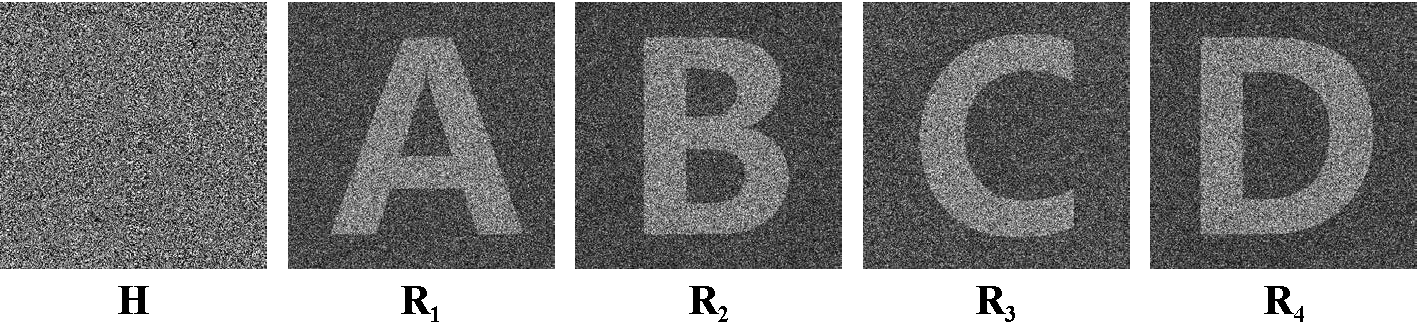
\includegraphics[width=1.0\textwidth]{ABCD/Naive_ABCD.pdf}
	\caption{Phase Unwrapping with Superposition method's result on the 4-slice target}
	\label{fig:Naive_ABCD}
\end{figure}

The simulation results shown in \cref{fig:Naive_ABCD} demonstrates the effectiveness of the Phase Unwrapping method. The reconstructions at each depth are legible, despite the presence of some noise. However, after applying a binary-phase quantisation on the hologram, the reconstruction quality deteriorates significantly, as shown in \cref{fig:Naive_ABCD_binary}.

\begin{figure}[H]
	\centering
	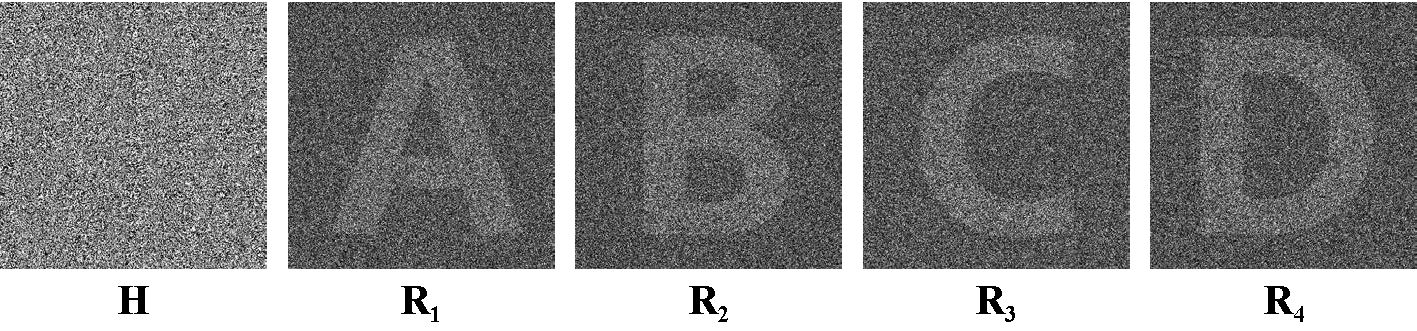
\includegraphics[width=1.0\textwidth]{ABCD/Naive_ABCD_binary.pdf}
	\caption{Phase Unwrapping method's result on the 4-slice target after binary quantisation}
	\label{fig:Naive_ABCD_binary}
\end{figure}

To improve the reconstruction quality, the time-multiplexed OSPR algorithm (in \cref{sec:One Step Phase Retrieval (OSPR) Algorithm}) is adapted to produce multi-frame holograms for 3D targets.


\subsubsection{OSPR algorithm adaptation}
\begin{figure}[H]
	\centering
	\includegraphics[width=1.0\textwidth]{ABCD/OSPR_ABCD.pdf}
	\caption{OSPR algorithm's result on the 4-slice target}
	\label{fig:OSPR_ABCD}
\end{figure}

The OSPR algorithm in \cref{sec:One Step Phase Retrieval (OSPR) Algorithm} was adapted to generate multi-depth targets by doing the Phase Unwrapping method in the previous paragraph for a total of $S$ times to form $S$ sub-frames. The results of the example run with $S=24$ is shown in \cref{fig:OSPR_ABCD}. The average reconstruction has much less noise than the single frame one in \cref{fig:Naive_ABCD_binary}. However, the contrast is not high enough. Therefore, one of the major objective of this thesis is to search for time-multiplexed binary-phase holograms with better reconstruction quality than the existing methods, which will be further explored in \cref{chapter:Multi Frame Holograms Batched Optimisation}.

\subsubsection{GS algorithm adaptations} \label{sec:GS algorithm adaptation}
The GS algorithm in \cref{sec:Gerchberg-Saxton (GS) Algorithm} can also be adapted to generate phase-only holograms for multi-depth 3D targets. Three different adaptations are reviewed in the following paragraphs.

\textbf{GS algorithm adaptation 1 - Superposition: }
Similar to the OSPR adaptation, the first method of adapting the GS algorithm for 3D CGH is by superposition. Firstly, a set of holograms are generated individually using the GS algorithm on each slice of the 3D target, and then those holograms are superposed into a total hologram whose phase is then unwrapped to be the final phase hologram.

\begin{figure}[H]
  \centering
  \includegraphics[width=1.0\textwidth]{ABCD/GS_noSS_ABCD.pdf}
  \caption{GS with superposition method's result on the 4-slice target}
  \label{fig:GS_noSS_ABCD}
\end{figure}

The GS with superposition method was run on the target field in \cref{fig:ABCD_target} and produced the result in \cref{fig:GS_noSS_ABCD}. Similar to the observations with the OSPR adaptation, the superposition leads to defocusing between each slice, giving rise to the background noise. The advantage of this method is its simplicity of implementation, while the disadvantages of this method are its poor reconstruction quality and its high number of iterations, which grows linearly with the number of slices.


\textbf{GS algorithm adaptation 2 - GS with Sequential Slicing (GS-SS): }
The second adaptation is called GS-SS, Instead of propagating to a fixed target image at each iteration, the GS algorithm is modified to propagate to a different distance at each iteration, and the target amplitude constraint of the according distance is applied (i.e. line $E \gets \sqrt{T} \times e^{j\angle E}$ in \cref{alg:Gerchberg-Saxton (GS) Algorithm} becomes $E \gets \sqrt{T_{i\%n}} \times e^{j\angle E}$, where $i$ is the iteration number, $n$ is the total number of slices and the $\%$ sign takes the remainder of the division). Such method is named sequential slicing, where the algorithm sweeps through the slices one by one sequentially during its iterations.

\begin{figure}[H]
  \centering
  \includegraphics[width=1.0\textwidth]{ABCD/GS_SS_ABCD.pdf}
  \caption{GS with sequential slicing algorithm's result on the 4-slice target}
  \label{fig:GS_SS_ABCD}
\end{figure}

The GS with sequential slicing (SS) algorithm was run on the target field in \cref{fig:ABCD_target} for 100 iterations, and the result is shown in \cref{fig:GS_SS_ABCD}. The interesting phenomena is that, as the 100 iterations terminated at the $4^{th}$ layer, the $4^{th}$ reconstruction ($R_4$) has the best quality among all slices, and the reconstruction quality deteriorates as the slice index reduces.

\begin{figure}[H]
  \centering
  \includegraphics[width=0.9\textwidth]{ABCD/Each_slice_GS.pdf}
  \caption{GS with SS algorithm's NMSE v.s. iteration number plot}
  \label{fig:Each_slice_GS}
\end{figure}

As a further investigation, the NMSE of each slice is plotted against iteration number in \cref{fig:Each_slice_GS}. It shows that the iterations did not converge. The NMSE curves are oscillating severely. When the NMSE of one slice decreases, the NMSE of all other slices increases. Applying the amplitude constraint at a single depth worsen all the other slices. There is a solution to this issue in the literature, called Dynamic Compensatory GS (DCGS) \cite{Zhou2019}, as introduced in the following paragraph.


\textbf{GS algorithm adaptation 3 - Dynamic Compensatory GS (DCGS): }
The DCGS algorithm `softens' the target field amplitude constraint \cite{Zhou2019}. Instead of forcing the amplitude of the reconstructed field to the target amplitude directly, it allows a fraction $\alpha$ of the original amplitude to be retained (i.e. $E \gets \sqrt{T_{i\%n}} \times e^{j\angle E}$ becomes $E \gets [\alpha \times \vert E \vert + (1-\alpha) \times \sqrt{T_{i\%n}}] \times e^{j\angle E}$), where $\alpha$ is adjusted dynamically at each iteration. The DCGS algorithm was implemented and run on the 4-slice target in \cref{fig:ABCD_target}. The result is shown in \cref{fig:DCGS_ABCD}.

\begin{figure}[H]
  \centering
  \includegraphics[width=1.0\textwidth]{ABCD/DCGS_ABCD.pdf}
  \caption{DCGS algorithm's result on the 4-slice target}
  \label{fig:DCGS_ABCD}
\end{figure}

\cref{fig:DCGS_ABCD} shows the effectiveness of the DCGS algorithm, where all slices have good quality instead of the huge inter-slice quality imbalance observed in \cref{fig:GS_SS_ABCD}. The NMSE of each slice is plotted against the iteration number in \cref{fig:Each_slice_DCGS}.

\begin{figure}[H]
  \centering
  \includegraphics[width=0.9\textwidth]{ABCD/Each_slice_DCGS.pdf}
  \caption{DCGS algorithm's NMSE v.s. iteration number plot}
  \label{fig:Each_slice_DCGS}
\end{figure}

\cref{fig:Each_slice_DCGS} shows a much better convergence than \cref{fig:Each_slice_GS}. Although the bounce-backs still present (i.e. when the NMSE of one slice decreases, those of other slices increase), the overall trend of NMSE is decreasing as the iterations continue.
